\chapter{Beyond variance reduction}
% \vspace{1em}

% TODO: table of contents of the appendix, renumeroter les propositions

\section*{Organization of the appendix}

We organize the appendix into several thematic sections. 

The first one, section \ref{app:exp} contains additional experiments and figures on bandits and MDPs. 
We have further investigations into committal and non-committal behaviour with baselines. 
More precisely subsection~\ref{app:exp_3armbandit} contains additional experiments for the 3 arm bandits for vanilla policy gradient, natural policy gradient and policy gradient with direct parameterization and a discussion on the effect the hyperparameters have on the results. In all cases, we find evidence for committal and non-committal behaviours. 
In the rest of the section, we investigate this in MDPs, starting with a smaller MDP with 2 different goals in subsection~\ref{app:simple_mdp} and constant baselines. We also provide additional experiments on the 4 rooms environment in subsection~\ref{app:4rooms_mdp}, including the vanilla policy gradient and constant baselines with REINFORCE. 

Then, section~\ref{app:theory_2arm} contains theory for the two-armed bandit case, namely proofs of convergence to a suboptimal policy (Proposition~\ref{proposition_divergence} in Appendix~\ref{app:2arm_constant_baseline_div}) and an analysis of perturbed minimum-variance baselines (Proposition~\ref{prop:2armed-perturbedminvar} in Appendix~\ref{sec:appendix_perturbed_minvar}). For the latter, depending on the perturbation, we may have possible convergence to a suboptimal policy, convergence to the optimal policy in probability, or a weaker form of convergence to the optimal policy. Finally, we also show vanilla policy gradient converges to the optimal policy in probability regardless of the baseline in Appendix~\ref{app:2arm_vanilla_pg}. 

Section~\ref{app:theory_multiarm} contains the theory for multi-armed bandit, including the proof of theorem~\ref{proposition_threearmedbandit}. This theorem presents a counterexample to the idea that reducing variance always improves optimization. We show that there is baseline leading to reduced variance which may converge to a suboptimal policy with positive probability (see Appendix~\ref{app:3arm_minvar_baseline_div}) while there is another baseline with larger variance that converges to the optimal policy with probability $1$ (see Appendix~\ref{app:3arm_gap_baseline}).
We identify on-policy sampling as being a potential source of these convergence issues. We provide proofs of proposition~\ref{lem:main_off-policy_IS} in Appendix \ref{app:3arm_off_policy}, which shows convergence to the optimal policy in probability when using off-policy sampling with importance sampling.  

Finally, in section~\ref{app:other_results}, we provide derivations of miscellaneous, smaller results such as the calculation of the minimum-variance baseline (Appendix~\ref{app:optimal_baseline}), the natural policy gradient update for the softmax parameterization (Appendix~\ref{app:npg_softmax_bandit}) and the connection between the value function and the minimum-variance baseline  (Appendix~\ref{app:value_minvar_baseline}).

\section{Other experiments}
\label{app:exp}

\subsection{Three-armed bandit}
\label{app:exp_3armbandit}
In this subsection, we provide additional experiments on the three-armed bandit with natural and vanilla policy gradients for the softmax parameterization, varying the initializations.  Additionally, we present results for the direct parameterization and utilizing projected stochastic gradient ascent. 

The main takeaway is that the effect of the baselines appears more strongly when the initialization is unfavorable (for instance with a high probability of selecting a suboptimal action at first). The effect also are diminished when using small learning rates as in that case the effect of the noise on the optimization process lessens.

While the simplex visualization is very appealing, we mainly show here learning curves as we can showcase more seeds that way and show the effects are noticeable across many runs.

\subsubsection*{Natural policy gradient}
\begin{figure}[!ht]
\centering
  \begin{subfigure}[b]{0.245\linewidth}
    % 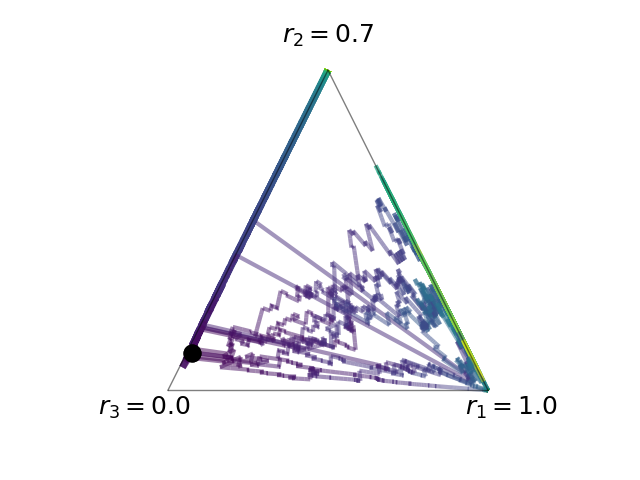
\includegraphics[trim={2cm 1.5cm 2cm
      % 0},clip,width=\textwidth]{articles/baselines/figs/simplex_plots/committal_ternary.png}
    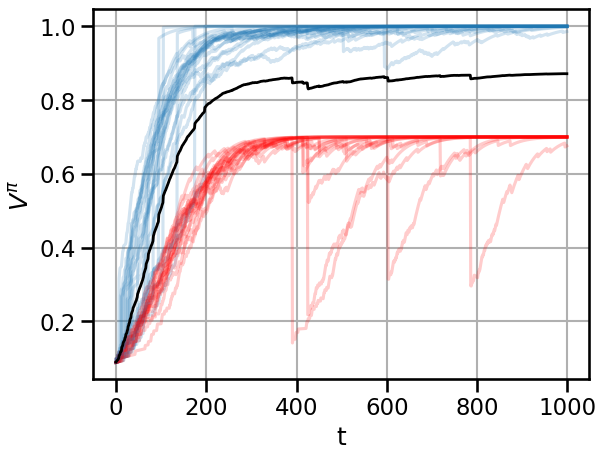
\includegraphics[width=\textwidth]{articles/baselines/figs/appendix_figs_3arm_035/natural_minvar_-05_eta=0025.png}
    \caption{$b = b^\ast - \nicefrac{1}{2}$}
  \end{subfigure}
%   \hfill
    \begin{subfigure}[b]{0.245\linewidth}
    % 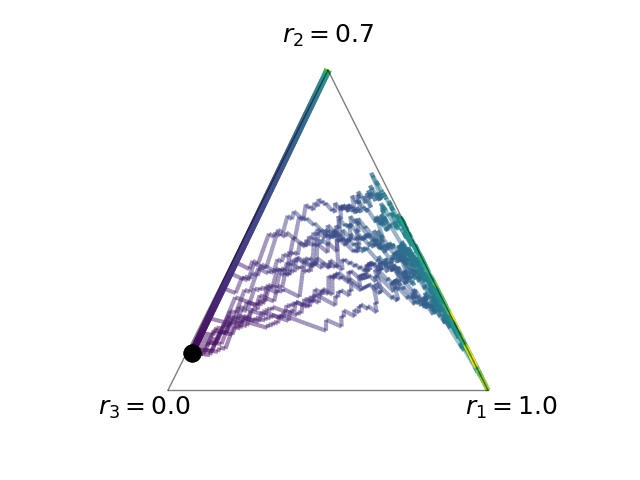
\includegraphics[trim={2cm 1.5cm 2cm
        % 0},clip,width=\textwidth]{articles/baselines/figs/simplex_plots/minvar_ternary.png}
    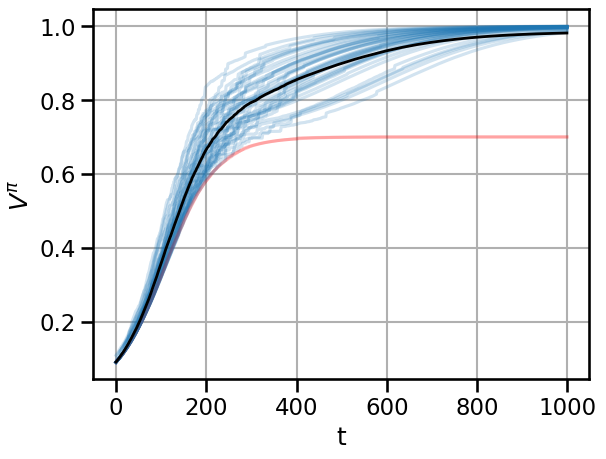
\includegraphics[width=\textwidth]{articles/baselines/figs/appendix_figs_3arm_035/natural_minvar_0_eta=0025.png}
    \caption{$b = b^\ast$}
  \end{subfigure}
  \begin{subfigure}[b]{0.245\linewidth}
    % 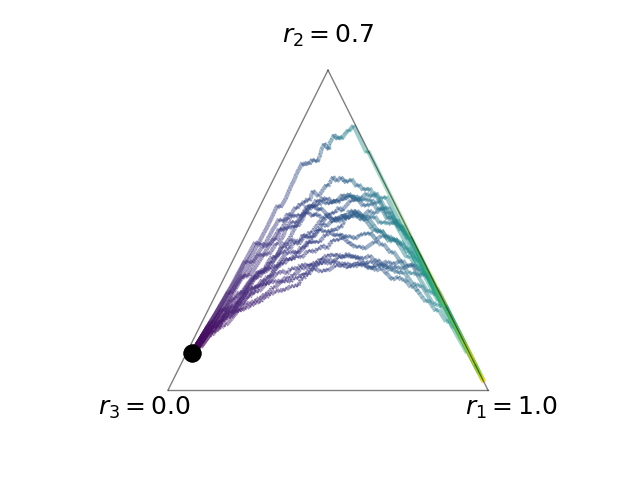
\includegraphics[trim={2cm 1.5cm 2cm
      % 0},clip,width=\textwidth]{articles/baselines/figs/simplex_plots/non_committal_ternary.png}
    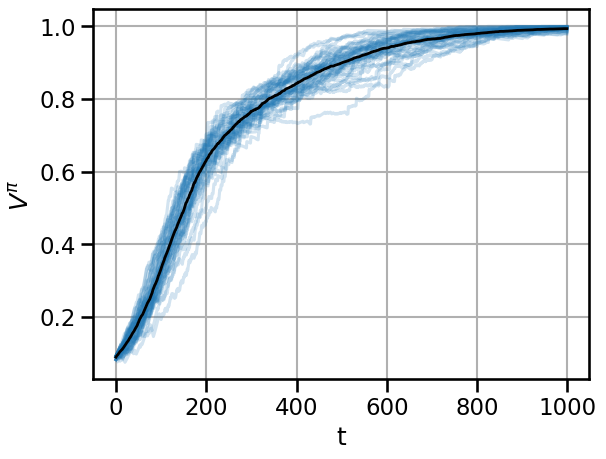
\includegraphics[width=\textwidth]{articles/baselines/figs/appendix_figs_3arm_035/natural_minvar_05_eta=0025.png}
    \caption{$b = b^\ast + \nicefrac{1}{2}$}
  \end{subfigure}
%   \hfill
  \begin{subfigure}[b]{0.245\linewidth}
    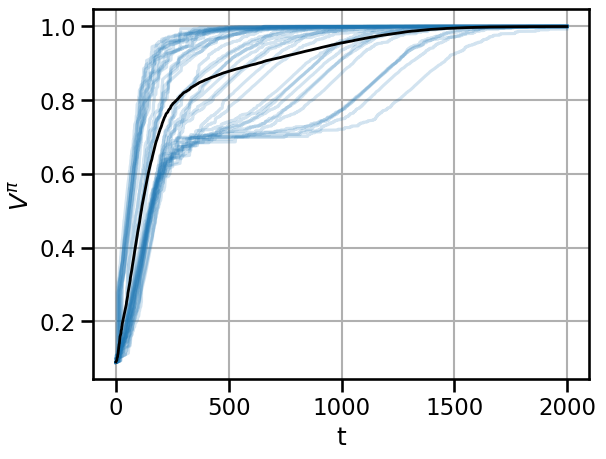
\includegraphics[width=\textwidth]{articles/baselines/figs/appendix_figs_3arm_035/natural_value_0_eta=0025.png}
    % 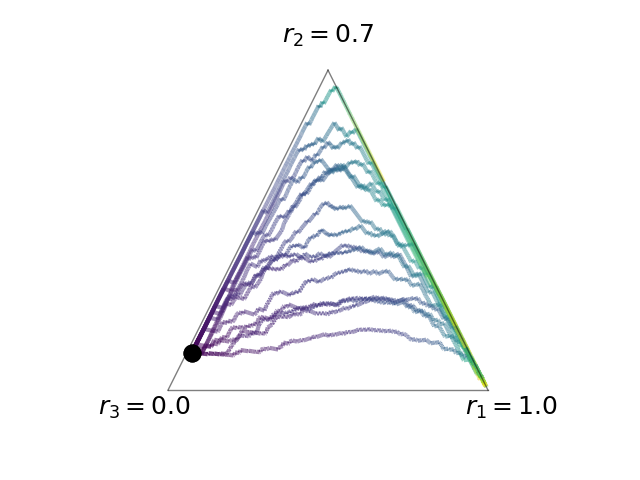
\includegraphics[trim={2cm 1.5cm 2cm
    % 0},clip,width=\textwidth]{articles/baselines/figs/simplex_plots/valuefunction_ternary.png}
    \caption{$b=V^\pi$}
  \end{subfigure}
  \caption{We plot 40 different learning curves (in blue and red) of natural policy gradient, when using various baselines, on a 3-arm bandit problem with rewards $(1, 0.7, 0)$, $\alpha = 0.025$ and $\theta_0 = (0, 3, 5)$. The black line is the average value over the 40 seeds for each setting. The red curves denote the seeds that did not reach a value of at least $0.9$ at the end of training. Note that the value function baseline convergence was slow and thus was trained for twice the number of time steps.}~\label{appfig:learning_curves_npg_035}
\end{figure}
Figure~\ref{appfig:learning_curves_npg_035} uses the same setting as Figure~\ref{fig:trajectories} with 40 trajectories instead of 15. We do once again observe many cases of convergence to the wrong arm for the negative baseline and some cases for the minimum variance baseline, while the positive baseline converges reliably. In this case the value function also converges to the optimal solution but is much slower.

\begin{figure}[!ht]
\centering
  \begin{subfigure}[b]{0.245\linewidth}
    % 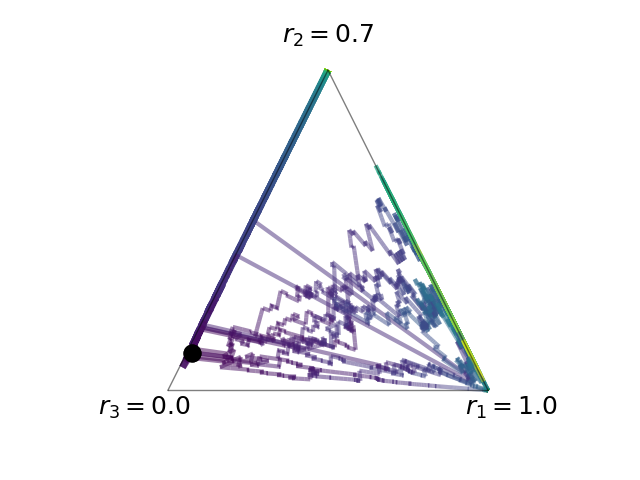
\includegraphics[trim={2cm 1.5cm 2cm
      % 0},clip,width=\textwidth]{articles/baselines/figs/simplex_plots/committal_ternary.png}
    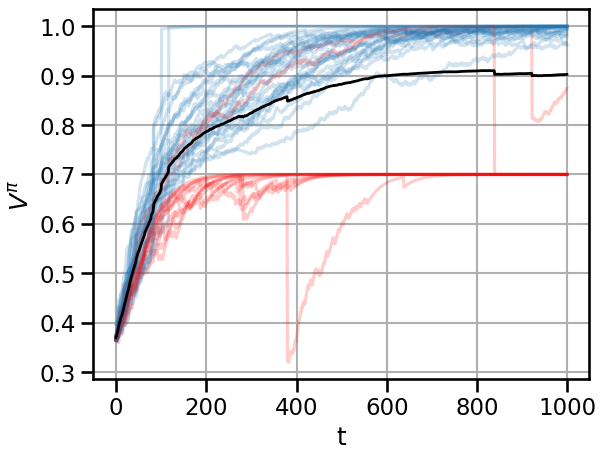
\includegraphics[width=\textwidth]{articles/baselines/figs/appendix_figs_3arm_033/natural_minvar_-05_eta=0025.png}
    \caption{$b = b^\ast - \nicefrac{1}{2}$}
  \end{subfigure}
%   \hfill
    \begin{subfigure}[b]{0.245\linewidth}
    % 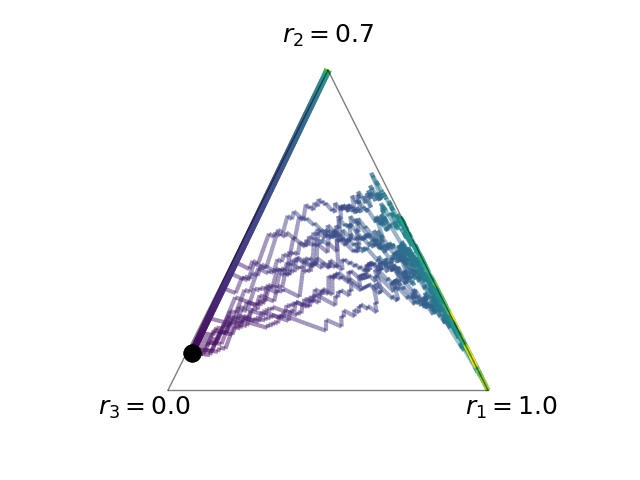
\includegraphics[trim={2cm 1.5cm 2cm
        % 0},clip,width=\textwidth]{articles/baselines/figs/simplex_plots/minvar_ternary.png}
    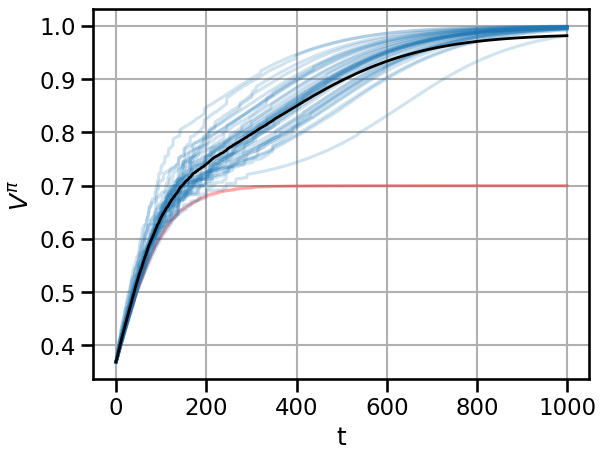
\includegraphics[width=\textwidth]{articles/baselines/figs/appendix_figs_3arm_033/natural_minvar_0_eta=0025.png}
    \caption{$b = b^\ast$}
  \end{subfigure}
  \begin{subfigure}[b]{0.245\linewidth}
    % 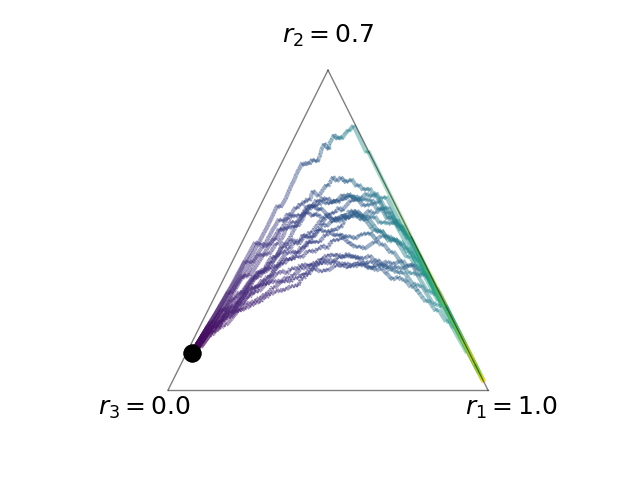
\includegraphics[trim={2cm 1.5cm 2cm
      % 0},clip,width=\textwidth]{articles/baselines/figs/simplex_plots/non_committal_ternary.png}
    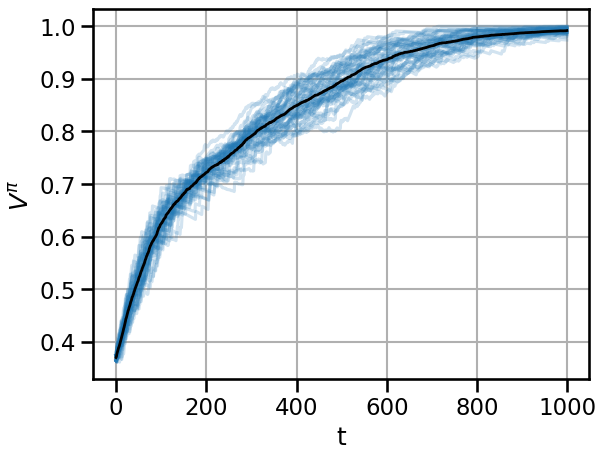
\includegraphics[width=\textwidth]{articles/baselines/figs/appendix_figs_3arm_033/natural_minvar_05_eta=0025.png}
    \caption{$b = b^\ast + \nicefrac{1}{2}$}
  \end{subfigure}
%   \hfill
  \begin{subfigure}[b]{0.245\linewidth}
    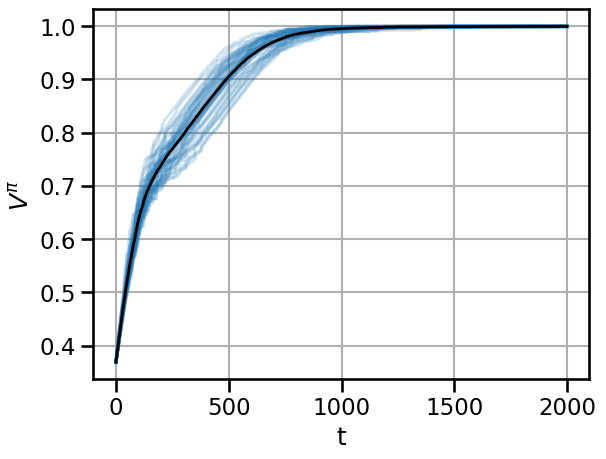
\includegraphics[width=\textwidth]{articles/baselines/figs/appendix_figs_3arm_033/natural_value_0_eta=0025.png}
    % 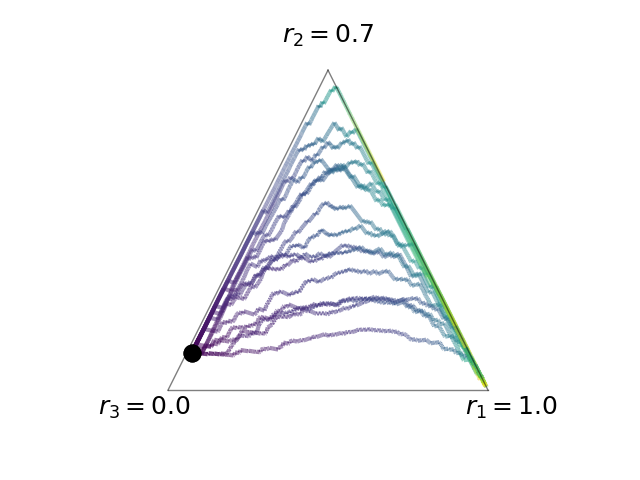
\includegraphics[trim={2cm 1.5cm 2cm
    % 0},clip,width=\textwidth]{articles/baselines/figs/simplex_plots/valuefunction_ternary.png}
    \caption{$b=V^\pi$}
  \end{subfigure}
  \caption{We plot 40 different learning curves (in blue and red) of natural policy gradient, when using various baselines, on a 3-arm bandit problem with rewards $(1, 0.7, 0)$, $\alpha = 0.025$ and $\theta_0 = (0, 3, 3)$. The black line is the average value over the 40 seeds for each setting. The red curves denote the seeds that did not reach a value of at least $0.9$ at the end of training.}~\label{appfig:learning_curves_npg_033}
\end{figure}
Figure~\ref{appfig:learning_curves_npg_033} shows a similar setting to Figure~\ref{appfig:learning_curves_npg_035} but where the initialization parameter is not as extreme. We observe the same type of behavior, but not as pronounced as before; fewer seeds converge to the wrong arm.


\begin{figure}[!ht]
\centering
  \begin{subfigure}[b]{0.245\linewidth}
    % 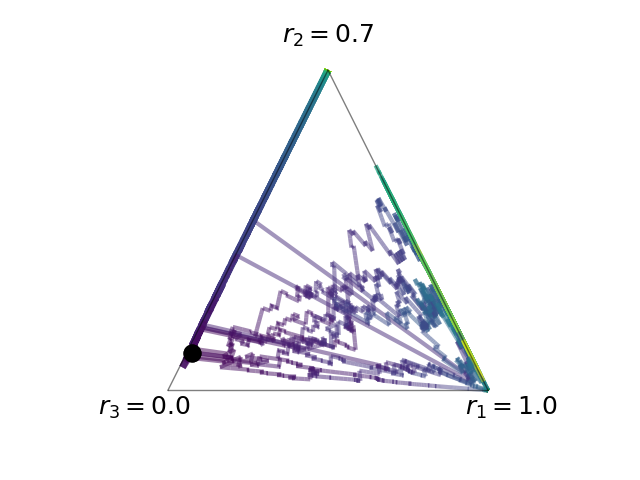
\includegraphics[trim={2cm 1.5cm 2cm
      % 0},clip,width=\textwidth]{articles/baselines/figs/simplex_plots/committal_ternary.png}
    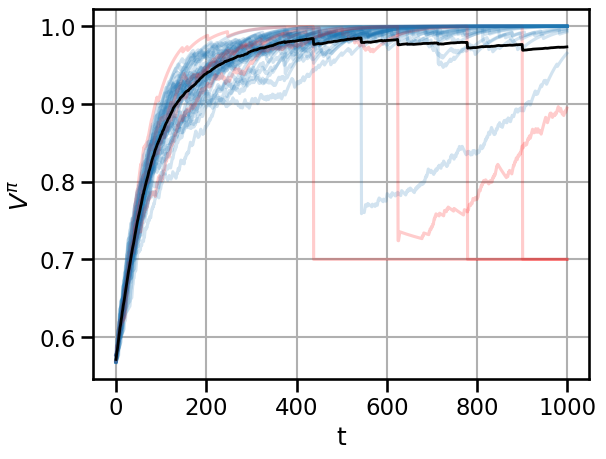
\includegraphics[width=\textwidth]{articles/baselines/figs/appendix_figs_3arm_000/natural_minvar_-05_eta=0025.png}
    \caption{$b = b^\ast - \nicefrac{1}{2}$}
  \end{subfigure}
%   \hfill
    \begin{subfigure}[b]{0.245\linewidth}
    % 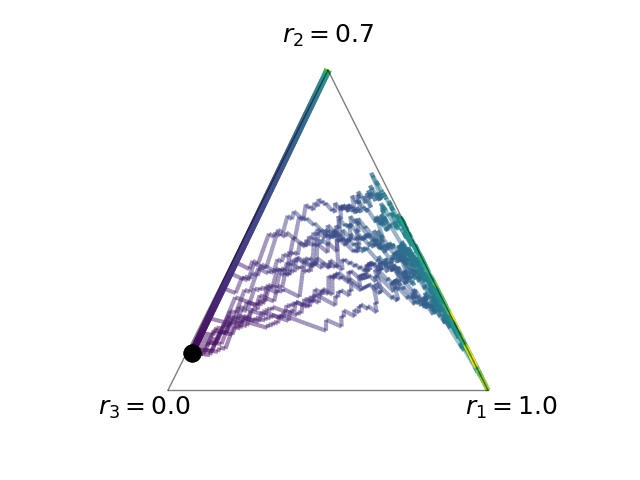
\includegraphics[trim={2cm 1.5cm 2cm
        % 0},clip,width=\textwidth]{articles/baselines/figs/simplex_plots/minvar_ternary.png}
    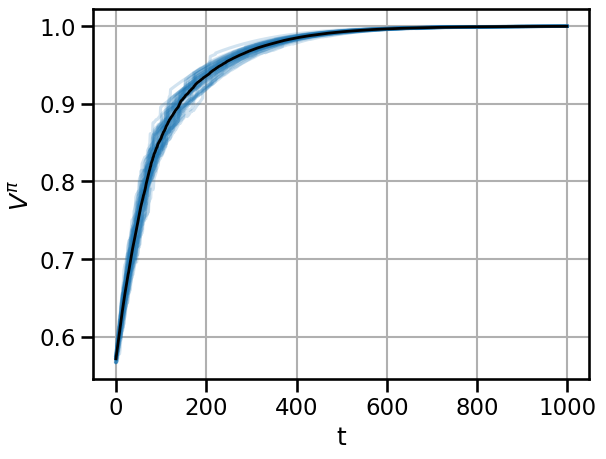
\includegraphics[width=\textwidth]{articles/baselines/figs/appendix_figs_3arm_000/natural_minvar_0_eta=0025.png}
    \caption{$b = b^\ast$}
  \end{subfigure}
  \begin{subfigure}[b]{0.245\linewidth}
    % 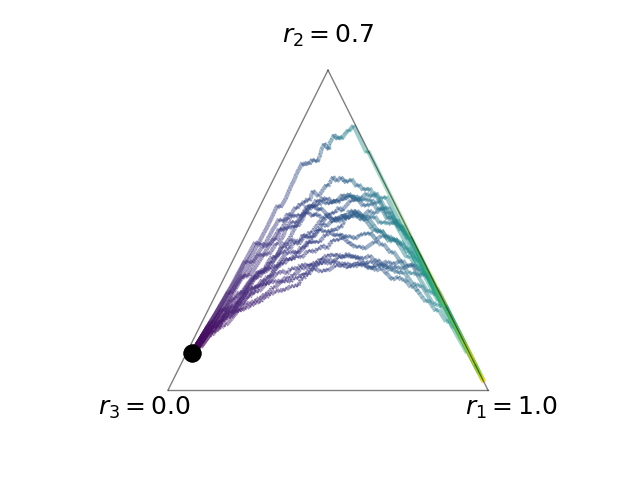
\includegraphics[trim={2cm 1.5cm 2cm
      % 0},clip,width=\textwidth]{articles/baselines/figs/simplex_plots/non_committal_ternary.png}
    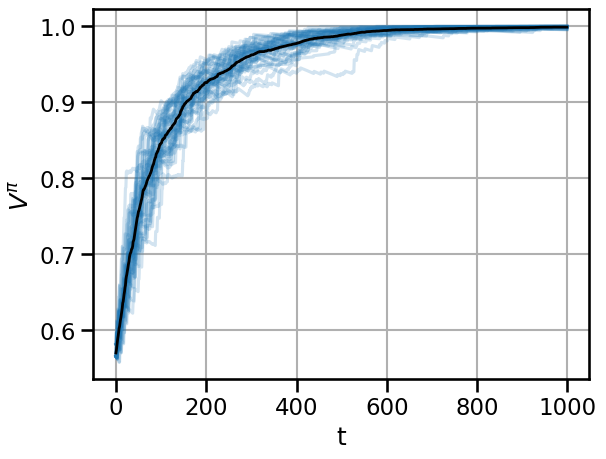
\includegraphics[width=\textwidth]{articles/baselines/figs/appendix_figs_3arm_000/natural_minvar_05_eta=0025.png}
    \caption{$b = b^\ast + \nicefrac{1}{2}$}
  \end{subfigure}
%   \hfill
  \begin{subfigure}[b]{0.245\linewidth}
    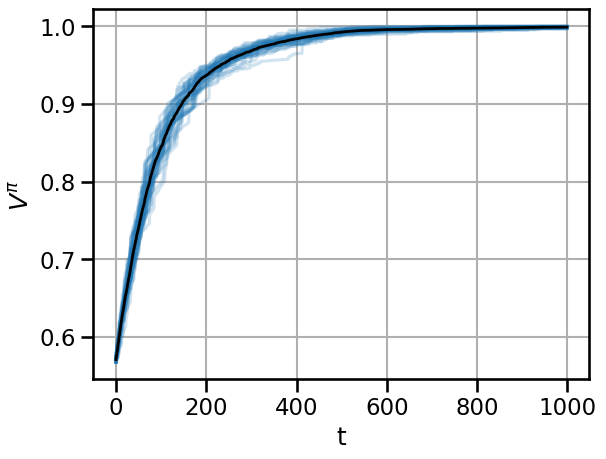
\includegraphics[width=\textwidth]{articles/baselines/figs/appendix_figs_3arm_000/natural_value_0_eta=0025.png}
    % 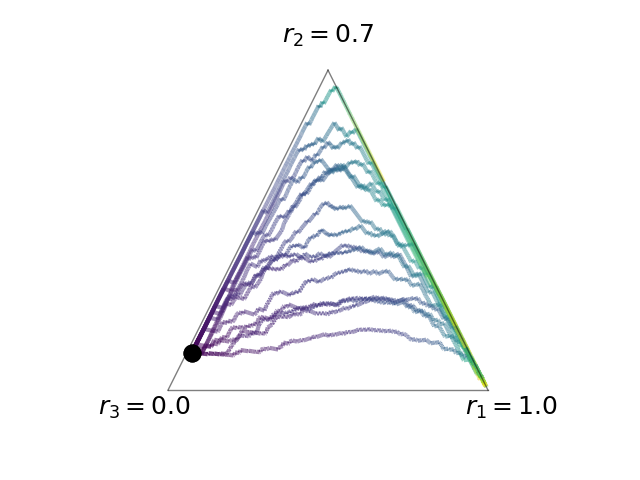
\includegraphics[trim={2cm 1.5cm 2cm
    % 0},clip,width=\textwidth]{articles/baselines/figs/simplex_plots/valuefunction_ternary.png}
    \caption{$b=V^\pi$}
  \end{subfigure}
  \caption{We plot 40 different learning curves (in blue and red) of natural policy gradient, when using various baselines, on a 3-arm bandit problem with rewards $(1, 0.7, 0)$, $\alpha = 0.025$ and $\theta_0 = (0, 0, 0)$ i.e the initial policy is uniform. The black line is the average value over the 40 seeds for each setting. The red curves denote the seeds that did not reach a value of at least $0.9$ at the end of training.}~\label{appfig:learning_curves_npg_000}
\end{figure}
In Figure~\ref{appfig:learning_curves_npg_000} whose initial policy is the uniform, we observe that the minimum variance baseline and the value function as baseline perform very well. On the other hand the committal baseline still has seeds that do not converge to the right arm. Interestingly, while all seeds for the non-committal baseline identify the optimal arm, the variance of the return is higher than for the optimal baseline, suggesting a case similar to the result presented in Proposition \ref{lem:prop_epsilon_1inf} where a positive baseline ensured we get close to the optimal arm but may not remain arbitrary close to it.


\subsubsection*{Vanilla policy gradient}
While we have no theory indicating that we may converge to a suboptimal arm with vanilla policy gradient, we can still observe some effect in terms of learning speed in practice (see Figures \ref{appfig:learning_curves_vpg_000_simplex} to \ref{appfig:learning_curves_vpg_033}). 

On Figures~\ref{appfig:learning_curves_vpg_000_simplex} and~\ref{appfig:learning_curves_vpg_000} we plot the simplex view and the learning curves for vanilla policy gradient initialized at the uniform policy. We do observe that some trajectories did not converge to the optimal arm in the imparted time for the committal baseline, while they converged in all other settings. The mininum variance baseline is slower to converge than the non-committal and the value function in this setting as can be seem both in the simplex plot and learning curves.

\begin{figure}[!ht]
\centering
  \begin{subfigure}[b]{0.245\linewidth}
    % 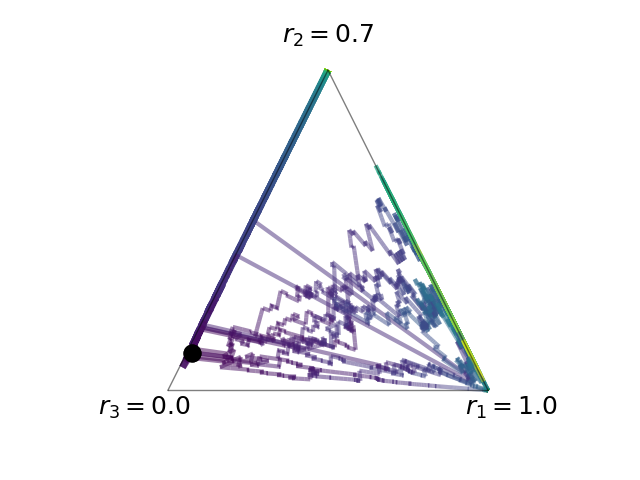
\includegraphics[trim={2cm 1.5cm 2cm
      % 0},clip,width=\textwidth]{articles/baselines/figs/simplex_plots/committal_ternary.png}
    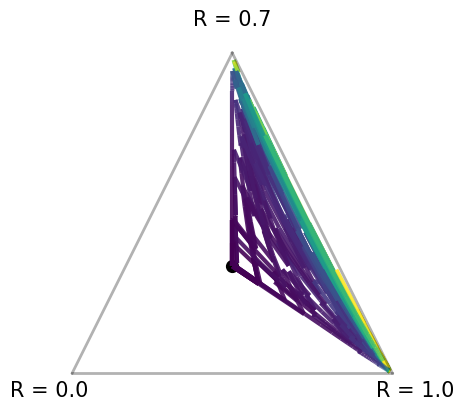
\includegraphics[width=\textwidth]{articles/baselines/figs/appendix_figs_3arm_000/vanilla_minvar_-05.png}
    \caption{$b = b^\ast - \nicefrac{1}{2}$}
  \end{subfigure}
%   \hfill
    \begin{subfigure}[b]{0.245\linewidth}
    % 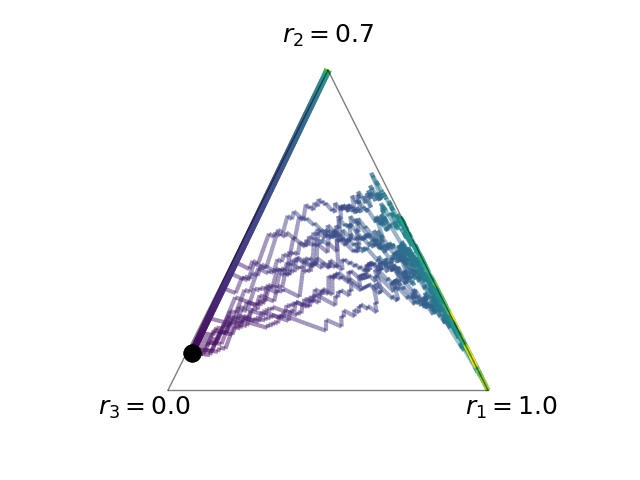
\includegraphics[trim={2cm 1.5cm 2cm
        % 0},clip,width=\textwidth]{articles/baselines/figs/simplex_plots/minvar_ternary.png}
    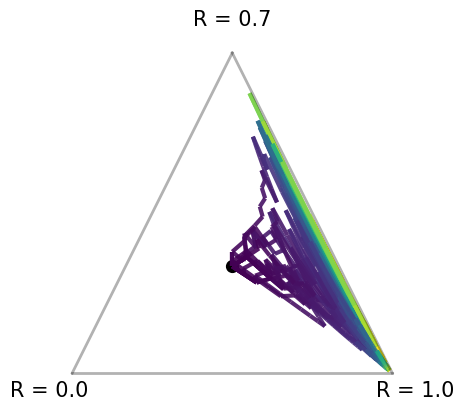
\includegraphics[width=\textwidth]{articles/baselines/figs/appendix_figs_3arm_000/vanilla_minvar_00.png}
    \caption{$b = b^\ast$}
  \end{subfigure}
  \begin{subfigure}[b]{0.245\linewidth}
    % 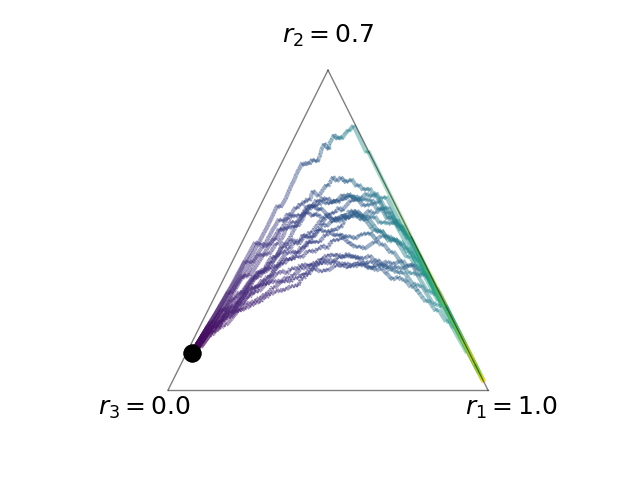
\includegraphics[trim={2cm 1.5cm 2cm
      % 0},clip,width=\textwidth]{articles/baselines/figs/simplex_plots/non_committal_ternary.png}
    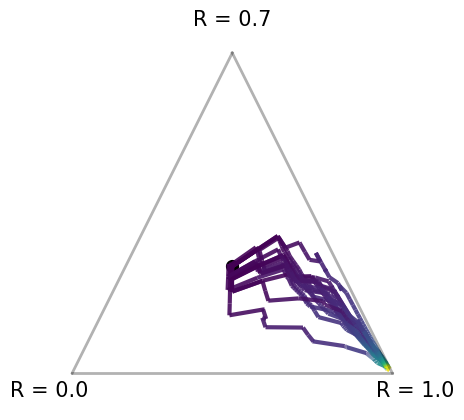
\includegraphics[width=\textwidth]{articles/baselines/figs/appendix_figs_3arm_000/vanilla_minvar_05.png}
    \caption{$b = b^\ast + \nicefrac{1}{2}$}
  \end{subfigure}
%   \hfill
  \begin{subfigure}[b]{0.245\linewidth}
    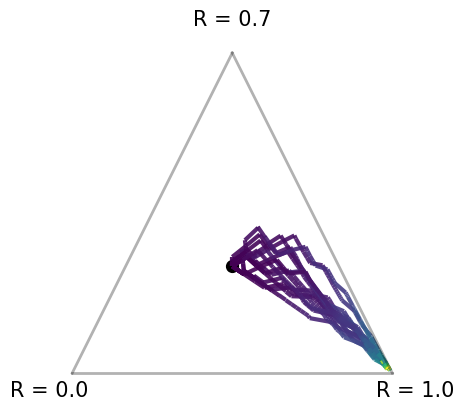
\includegraphics[width=\textwidth]{articles/baselines/figs/appendix_figs_3arm_000/vanilla_value_00.png}
    % 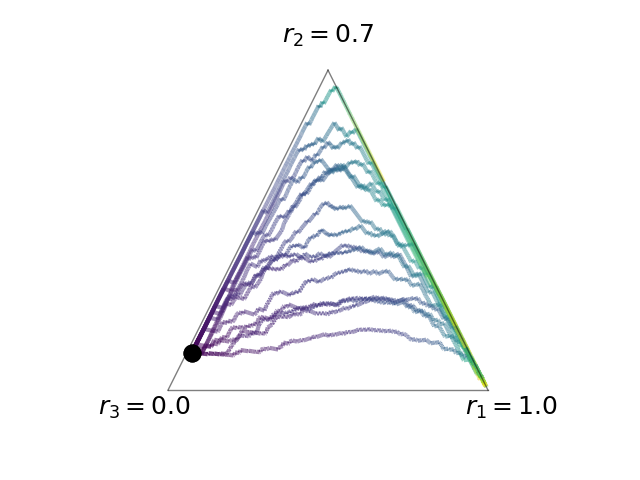
\includegraphics[trim={2cm 1.5cm 2cm
    % 0},clip,width=\textwidth]{articles/baselines/figs/simplex_plots/valuefunction_ternary.png}
    \caption{$b=V^\pi$}
  \end{subfigure}
  \caption{Simplex plot of 15 different learning curves for vanilla policy gradient, when using various baselines, on a 3-arm bandit problem with rewards $(1, 0.7, 0)$, $\alpha = 0.5$ and $\theta_0 = (0, 0, 0)$. Colors, from purple to yellow represent training steps.}~\label{appfig:learning_curves_vpg_000_simplex}
\end{figure}

\begin{figure}[!ht]
\centering
  \begin{subfigure}[b]{0.245\linewidth}
    % 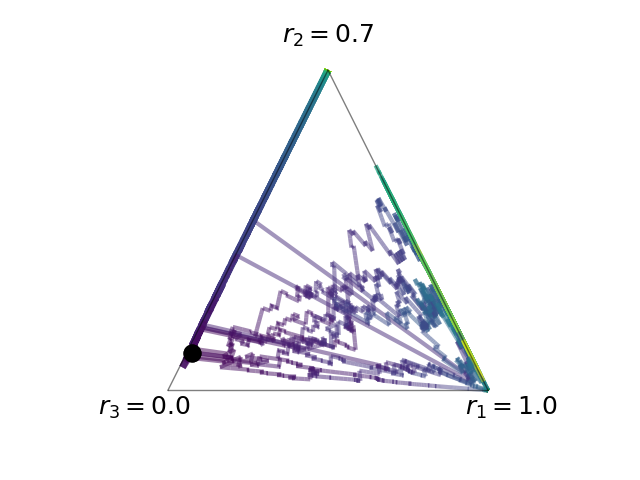
\includegraphics[trim={2cm 1.5cm 2cm
      % 0},clip,width=\textwidth]{articles/baselines/figs/simplex_plots/committal_ternary.png}
    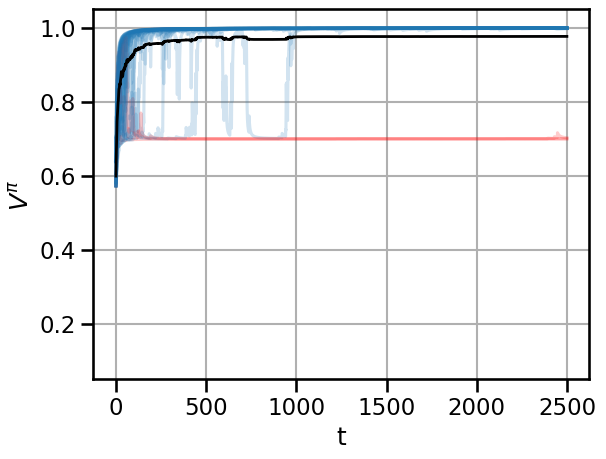
\includegraphics[width=\textwidth]{articles/baselines/figs/appendix_figs_3arm_000/vanilla_minvar_-05_eta=05.png}
    \caption{$b = b^\ast - \nicefrac{1}{2}$}
  \end{subfigure}
%   \hfill
    \begin{subfigure}[b]{0.245\linewidth}
    % 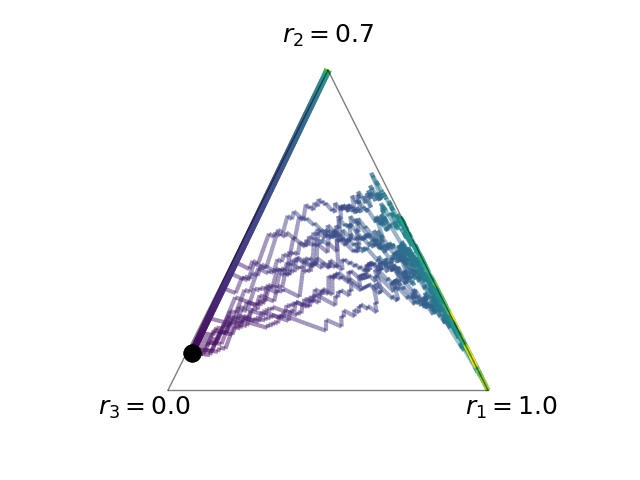
\includegraphics[trim={2cm 1.5cm 2cm
        % 0},clip,width=\textwidth]{articles/baselines/figs/simplex_plots/minvar_ternary.png}
    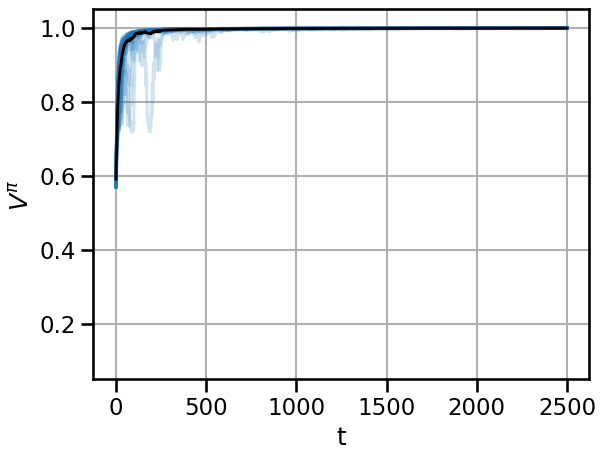
\includegraphics[width=\textwidth]{articles/baselines/figs/appendix_figs_3arm_000/vanilla_minvar_0_eta=05.png}
    \caption{$b = b^\ast$}
  \end{subfigure}
  \begin{subfigure}[b]{0.245\linewidth}
    % 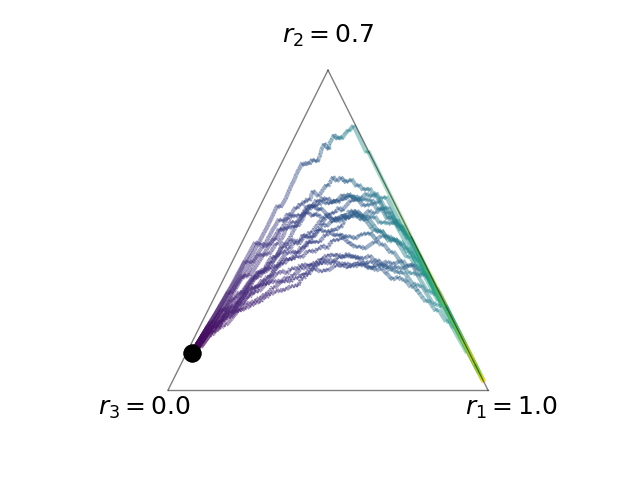
\includegraphics[trim={2cm 1.5cm 2cm
      % 0},clip,width=\textwidth]{articles/baselines/figs/simplex_plots/non_committal_ternary.png}
    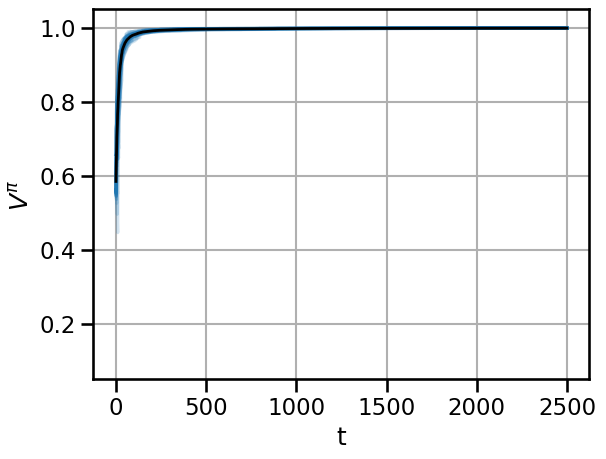
\includegraphics[width=\textwidth]{articles/baselines/figs/appendix_figs_3arm_000/vanilla_minvar_05_eta=05.png}
    \caption{$b = b^\ast + \nicefrac{1}{2}$}
  \end{subfigure}
%   \hfill
  \begin{subfigure}[b]{0.245\linewidth}
    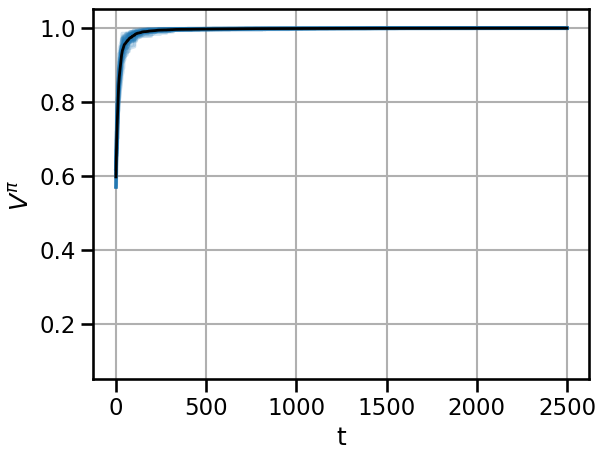
\includegraphics[width=\textwidth]{articles/baselines/figs/appendix_figs_3arm_000/vanilla_value_0_eta=05.png}
    % 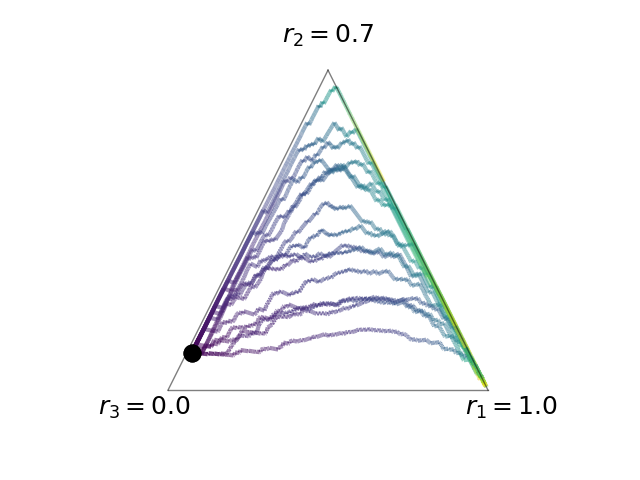
\includegraphics[trim={2cm 1.5cm 2cm
    % 0},clip,width=\textwidth]{articles/baselines/figs/simplex_plots/valuefunction_ternary.png}
    \caption{$b=V^\pi$}
  \end{subfigure}
  \caption{We plot 40 different learning curves (in blue and red) of vanilla policy gradient, when using various baselines, on a 3-arm bandit problem with rewards $(1, 0.7, 0)$, $\alpha = 0.5$ and $\theta_0 = (0, 0, 0)$. The black line is the average value over the 40 seeds for each setting. The red curves denote the seeds that did not reach a value of at least $0.9$ at the end of training.}~\label{appfig:learning_curves_vpg_000}
\end{figure}

On Figures~\ref{appfig:learning_curves_vpg_033_simplex} and~\ref{appfig:learning_curves_vpg_033} we plot the simplex view and the learning curves for vanilla policy gradient initialized at a policy yielding a very high probability of sampling the suboptimal actions, $48.7 \%$ for each. We do observe a similar behavior than for the previous plots with vanilla PG, but in this setting the minimum variance baseline is even slower to converge and a few seeds did not identify the optimal arm. As the gradient flow leads the solutions closer to the simplex edges, the simplex plot is not as helpful in this setting to understand the behavior of each baseline option.

\begin{figure}[!ht]
\centering
  \begin{subfigure}[b]{0.245\linewidth}
    % 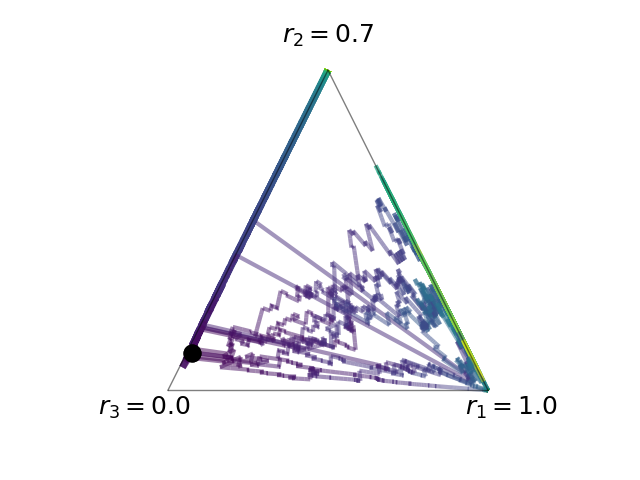
\includegraphics[trim={2cm 1.5cm 2cm
      % 0},clip,width=\textwidth]{articles/baselines/figs/simplex_plots/committal_ternary.png}
    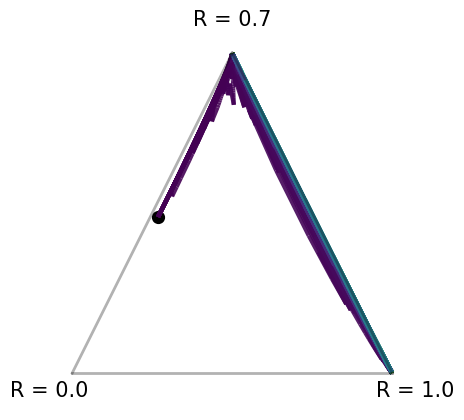
\includegraphics[width=\textwidth]{articles/baselines/figs/appendix_figs_3arm_033/vanilla_minvar_-05.png}
    \caption{$b = b^\ast - \nicefrac{1}{2}$}
  \end{subfigure}
%   \hfill
    \begin{subfigure}[b]{0.245\linewidth}
    % 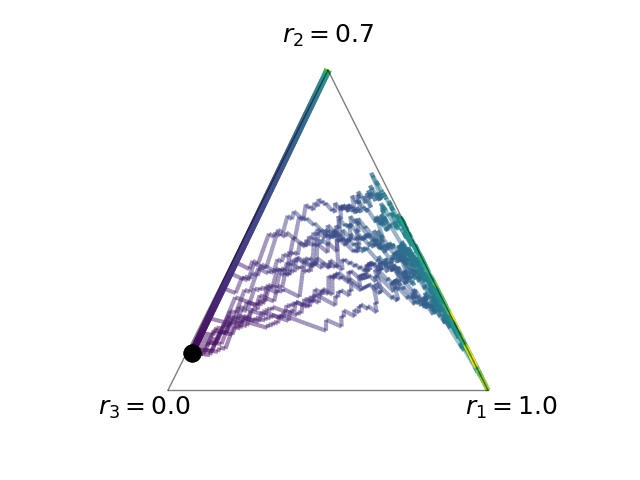
\includegraphics[trim={2cm 1.5cm 2cm
        % 0},clip,width=\textwidth]{articles/baselines/figs/simplex_plots/minvar_ternary.png}
    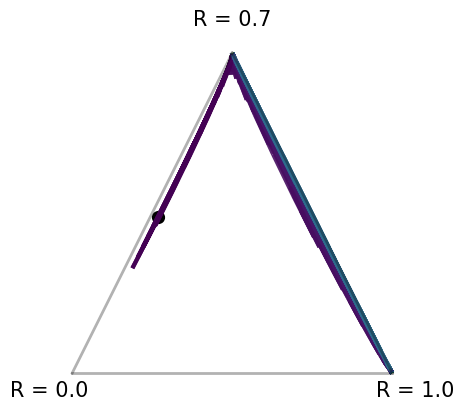
\includegraphics[width=\textwidth]{articles/baselines/figs/appendix_figs_3arm_033/vanilla_minvar_00.png}
    \caption{$b = b^\ast$}
  \end{subfigure}
  \begin{subfigure}[b]{0.245\linewidth}
    % 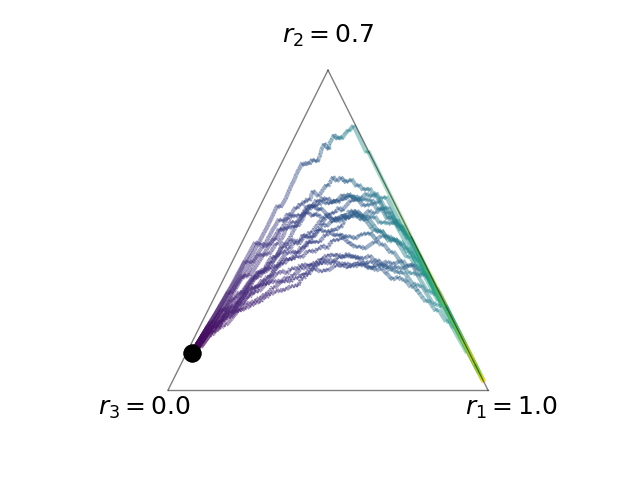
\includegraphics[trim={2cm 1.5cm 2cm
      % 0},clip,width=\textwidth]{articles/baselines/figs/simplex_plots/non_committal_ternary.png}
    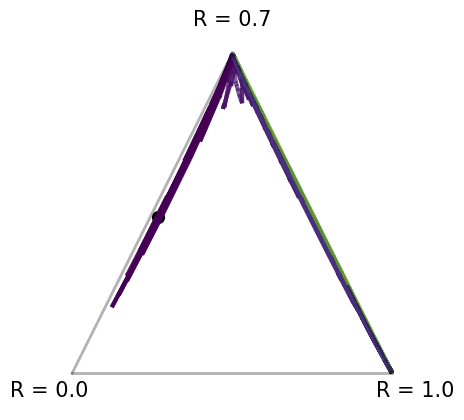
\includegraphics[width=\textwidth]{articles/baselines/figs/appendix_figs_3arm_033/vanilla_minvar_05.png}
    \caption{$b = b^\ast + \nicefrac{1}{2}$}
  \end{subfigure}
%   \hfill
  \begin{subfigure}[b]{0.245\linewidth}
    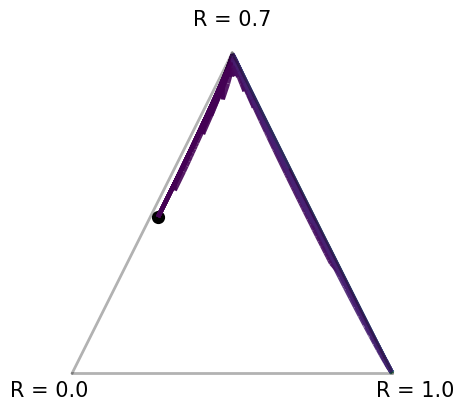
\includegraphics[width=\textwidth]{articles/baselines/figs/appendix_figs_3arm_033/vanilla_value_00.png}
    % 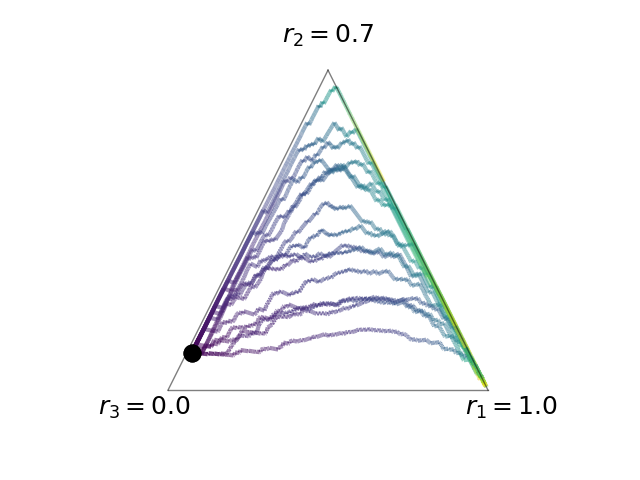
\includegraphics[trim={2cm 1.5cm 2cm
    % 0},clip,width=\textwidth]{articles/baselines/figs/simplex_plots/valuefunction_ternary.png}
    \caption{$b=V^\pi$}
  \end{subfigure}
  \caption{Simplex plot of 15 different learning curves for vanilla policy gradient, when using various baselines, on a 3-arm bandit problem with rewards $(1, 0.7, 0)$, $\alpha = 0.5$ and $\theta_0 = (0, 3, 3)$. Colors, from purple to yellow represent training steps.}~\label{appfig:learning_curves_vpg_033_simplex}
\end{figure}

\begin{figure}[!ht]
\centering
  \begin{subfigure}[b]{0.245\linewidth}
    % 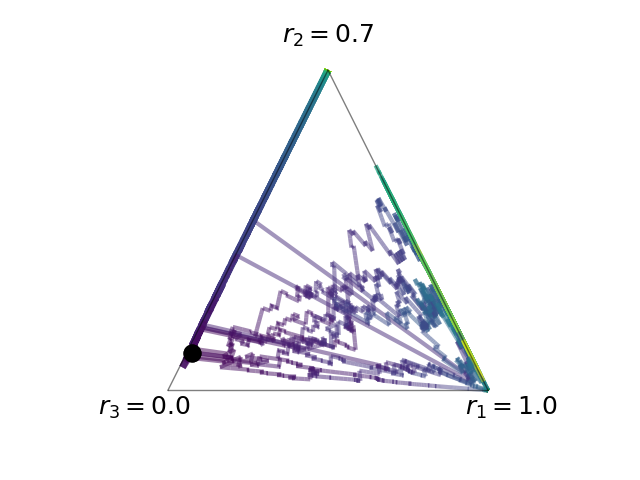
\includegraphics[trim={2cm 1.5cm 2cm
      % 0},clip,width=\textwidth]{articles/baselines/figs/simplex_plots/committal_ternary.png}
    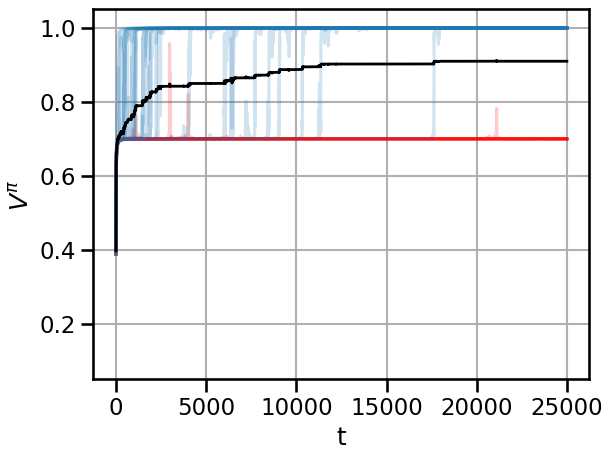
\includegraphics[width=\textwidth]{articles/baselines/figs/appendix_figs_3arm_033/vanilla_minvar_-05_eta=05.png}
    \caption{$b = b^\ast - \nicefrac{1}{2}$}
  \end{subfigure}
%   \hfill
    \begin{subfigure}[b]{0.245\linewidth}
    % \includegraphics[trim={2cm 1.5cm 2cm
        % 0},clip,width=\textwidth]{articles/baselines/figs/simplex_plots/minvar_ternary.png}
    \includegraphics[width=\textwidth]{articles/baselines/figs/appendix_figs_3arm_033/vanilla_minvar_0_eta=05.png}
    \caption{$b = b^\ast$}
  \end{subfigure}
  \begin{subfigure}[b]{0.245\linewidth}
    % \includegraphics[trim={2cm 1.5cm 2cm
      % 0},clip,width=\textwidth]{articles/baselines/figs/simplex_plots/non_committal_ternary.png}
    \includegraphics[width=\textwidth]{articles/baselines/figs/appendix_figs_3arm_033/vanilla_minvar_05_eta=05.png}
    \caption{$b = b^\ast + \nicefrac{1}{2}$}
  \end{subfigure}
%   \hfill
  \begin{subfigure}[b]{0.245\linewidth}
    \includegraphics[width=\textwidth]{articles/baselines/figs/appendix_figs_3arm_033/vanilla_value_0_eta=05.png}
    % \includegraphics[trim={2cm 1.5cm 2cm
    % 0},clip,width=\textwidth]{articles/baselines/figs/simplex_plots/valuefunction_ternary.png}
    \caption{$b=V^\pi$}
  \end{subfigure}
  \caption{We plot 40 different learning curves (in blue and red) of vanilla policy gradient, when using various baselines, on a 3-arm bandit problem with rewards $(1, 0.7, 0)$, $\alpha = 0.5$ and $\theta_0 = (0, 3, 3)$. The black line is the average value over the 40 seeds for each setting. The red curves denote the seeds that did not reach a value of at least $0.9$ at the end of training.}~\label{appfig:learning_curves_vpg_033}
\end{figure}




\subsubsection*{Policy gradient with direct parameterization}

Here we present results with the direct parameterization, i.e where $\theta$ contains directly the probability of drawing each arm. In that case the gradient update is
\begin{align*}
    \theta_{t+1} &= \text{Proj}_{\Delta_3} \big[ \theta_t + \alpha \frac{r(a_i)-b}{\theta(a_i)} \mathbf{1}_{a_i} \big]
\end{align*}
where $\Delta_3$ is the three dimensional simplex $\Delta_3 = \{u, v, w \ge 0, u+v+w = 1\}$. In this case, however, because the projection step is non trivial and doesn't have an easy explicit closed form solution (but we can express it as the output of an algorithm), we cannot explicitly write down the optimal baseline. Again, because of the projection step, baselines of this form are not guaranteed to preserve unbiasedness of the gradient estimate. For this reason, we only show experiments with fixed baselines, but keep in mind that these results are not as meaningful as the ones presented above. We present the results in Figures~\ref{appfig:learning_curves_dpg_035_simplex} and~\ref{appfig:learning_curves_dpg_035}.

\begin{figure}[!ht]
\centering
  \begin{subfigure}[b]{0.3\linewidth}
    % \includegraphics[trim={2cm 1.5cm 2cm
      % 0},clip,width=\textwidth]{articles/baselines/figs/simplex_plots/committal_ternary.png}
    \includegraphics[width=\textwidth]{articles/baselines/figs/appendix_figs_3arm_000/vanilla_fixed_-05.png}
    \caption{$b = - \nicefrac{1}{2}$}
  \end{subfigure}
%   \hfill
    \begin{subfigure}[b]{0.3\linewidth}
    % \includegraphics[trim={2cm 1.5cm 2cm
        % 0},clip,width=\textwidth]{articles/baselines/figs/simplex_plots/minvar_ternary.png}
    \includegraphics[width=\textwidth]{articles/baselines/figs/appendix_figs_3arm_000/vanilla_fixed_00.png}
    \caption{$b = 0$}
  \end{subfigure}
  \begin{subfigure}[b]{0.3\linewidth}
    % \includegraphics[trim={2cm 1.5cm 2cm
      % 0},clip,width=\textwidth]{articles/baselines/figs/simplex_plots/non_committal_ternary.png}
    \includegraphics[width=\textwidth]{articles/baselines/figs/appendix_figs_3arm_000/vanilla_fixed_05.png}
    \caption{$b = \nicefrac{1}{2}$}
  \end{subfigure}
  \caption{We plot 15 different learning curves of vanilla policy gradient with direct parameterization, when using various baselines, on a 3-arm bandit problem with rewards $(1, 0.7, 0)$, $\alpha = 0.1$ and $\theta_0 = (\nicefrac{1}{3}, \nicefrac{1}{3}, \nicefrac{1}{3})$, the uniform policy on the simplex.}~\label{appfig:learning_curves_dpg_035_simplex}
\end{figure}

\begin{figure}[!ht]
\centering
  \begin{subfigure}[b]{0.326\linewidth}
    % \includegraphics[trim={2cm 1.5cm 2cm
      % 0},clip,width=\textwidth]{articles/baselines/figs/simplex_plots/committal_ternary.png}
    \includegraphics[width=\textwidth]{articles/baselines/figs/appendix_figs_3arm_000/vanilla_fixed_-05_eta=01.png}
    \caption{$b = - \nicefrac{1}{2}$}
  \end{subfigure}
%   \hfill
    \begin{subfigure}[b]{0.326\linewidth}
    % \includegraphics[trim={2cm 1.5cm 2cm
        % 0},clip,width=\textwidth]{articles/baselines/figs/simplex_plots/minvar_ternary.png}
    \includegraphics[width=\textwidth]{articles/baselines/figs/appendix_figs_3arm_000/vanilla_fixed_00_eta=01.png}
    \caption{$b = 0$}
  \end{subfigure}
  \begin{subfigure}[b]{0.326\linewidth}
    % \includegraphics[trim={2cm 1.5cm 2cm
      % 0},clip,width=\textwidth]{articles/baselines/figs/simplex_plots/non_committal_ternary.png}
    \includegraphics[width=\textwidth]{articles/baselines/figs/appendix_figs_3arm_000/vanilla_fixed_05_eta=01.png}
    \caption{$b = \nicefrac{1}{2}$}
  \end{subfigure}
  \caption{We plot 40 different learning curves (in blue and red) of vanilla policy gradient with direct parameterization, when using various baselines, on a 3-arm bandit problem with rewards $(1, 0.7, 0)$, $\alpha = 0.1$ and $\theta_0 = (\nicefrac{1}{3}, \nicefrac{1}{3}, \nicefrac{1}{3})$, the uniform policy. The black line is the average value over the 40 seeds for each setting. The red curves denote the seeds that did not reach a value of at least $0.9$ at the end of training.}~\label{appfig:learning_curves_dpg_035}
\end{figure}

Once again in this setting we can see that negative baselines tend to encourage convergence to a suboptimal arm while positive baselines help converge to the optimal arm.



\subsubsection*{Policy gradient with escort transform parameterization}

We try the escort transform \cite{mei2020escaping} which was found to lead to better curvature properties of the objective than the softmax parameterization. We use the escort transform parameter $p=2$ as in the experiments for the original paper and find results similar to the softmax parameterization.
In fact, since this parameterization has larger updates near deterministic policies, it may be more prone to getting stuck at suboptimal policies when a choosing a committal baseline.

\begin{figure}[!ht]
\centering
  \begin{subfigure}[b]{0.3\linewidth}
    % \includegraphics[trim={2cm 1.5cm 2cm
      % 0},clip,width=\textwidth]{articles/baselines/figs/simplex_plots/committal_ternary.png}
    \includegraphics[width=\textwidth]{articles/baselines/figs/escort_transform/escort_vanilla_minvar_-05.png}
    \caption{$b = - \nicefrac{1}{2}$}
  \end{subfigure}
%   \hfill
    \begin{subfigure}[b]{0.3\linewidth}
    \includegraphics[width=\textwidth]{articles/baselines/figs/escort_transform/escort_vanilla_minvar_0.png}
    \caption{$b = 0$}
  \end{subfigure}
  \begin{subfigure}[b]{0.3\linewidth}
    \includegraphics[width=\textwidth]{articles/baselines/figs/escort_transform/escort_vanilla_minvar_05.png}
    \caption{$b = \nicefrac{1}{2}$}
  \end{subfigure}
  \caption{We plot 15 different learning curves of vanilla policy gradient with the escort transform with parameter $p=2$ \citep{mei2020escaping}, when using various baselines, on a 3-arm bandit problem with rewards $(1, 0.7, 0)$, $\alpha = 0.25$ and $\theta_0 = (1,1,1)$, the uniform policy on the simplex.}~\label{appfig:learning_curves_escort_simplex}
\end{figure}




\subsubsection*{Policy gradient with mellowmax parameterization}

As an alternate parameterization, we try the mellowmax function \cite{asadi2017alternative}.
Unfortunately, it is not trivial to utilize it with policy gradient methods.
The mellowmax algorithm was designed for SARSA as it requires Q-function estimates and the temperature parameter $\beta$ has to be computed using a black-box optimizer to find a maximum-entropy policy, thus cannot be differentiated through easily. However, using a naive version (treating $\beta$ as a constant in the policy gradient, setting $\omega = 1$ and using the parameters directly in place of Q), we observe that the committal vs. non-committal behaviors are greatly mitigated and all paths conserve a higher entropy and converge to the optimal arm. This strategy could be viewed as adding an entropy-regularizer with biased updates. Note that the baseline we used as the ``minimum-variance'' is not the true minimizer due to this bias too. Furthermore, even though the divergence is mitigated, the complexity per iteration rises significantly due to solving a black-box optimization problem at every step.


\begin{figure}[!ht]
\centering
  \begin{subfigure}[b]{0.3\linewidth}
    % \includegraphics[trim={2cm 1.5cm 2cm
      % 0},clip,width=\textwidth]{articles/baselines/figs/simplex_plots/committal_ternary.png}
    \includegraphics[width=\textwidth]{articles/baselines/figs/mellowmax_transform/vanilla_minvar_-05.png}
    \caption{$b = - \nicefrac{1}{2}$}
  \end{subfigure}
%   \hfill
    \begin{subfigure}[b]{0.3\linewidth}
    \includegraphics[width=\textwidth]{articles/baselines/figs/mellowmax_transform/vanilla_minvar_00.png}
    \caption{$b = 0$}
  \end{subfigure}
  \begin{subfigure}[b]{0.3\linewidth}
    \includegraphics[width=\textwidth]{articles/baselines/figs/mellowmax_transform/vanilla_minvar_05.png}
    \caption{$b = \nicefrac{1}{2}$}
  \end{subfigure}
  \caption{We plot 15 different learning curves of a policy gradient with the mellowmax transform \cite{asadi2017alternative}, when using various baselines, on a 3-arm bandit problem with rewards $(1, 0.7, 0)$, $\alpha = 0.25$ and $\theta_0 = (0,3,5)$.}~\label{appfig:learning_curves_mellowmax_simplex}
\end{figure}

% \subsection{3-armed bandits with natural policy gradient}
% We start by repeating the experiment in Section 2 with natural policy gradient instead of the vanilla policy gradient to emphasize that, although the theoretical results differ in both settings, empirical results are similar.

% \begin{figure}[!ht]
% \centering
%   \begin{subfigure}[b]{0.245\linewidth}
%     % \includegraphics[trim={2cm 1.5cm 2cm
%     0},clip,width=\textwidth]{articles/baselines/figs/simplex_plots/committal_ternary.png}
%     \includegraphics[width=\textwidth]{articles/baselines/figs/simplex_plots/simplex_traj_optimal_-1.png}
%     \caption{$b = b^\ast - 1$}
%   \end{subfigure}
% %   \hfill
%     \begin{subfigure}[b]{0.245\linewidth}
%     % \includegraphics[trim={2cm 1.5cm 2cm
%     0},clip,width=\textwidth]{articles/baselines/figs/simplex_plots/minvar_ternary.png}
%     \includegraphics[width=\textwidth]{articles/baselines/figs/simplex_plots/simplex_traj_optimal_0.png}
%     \caption{$b = b^\ast$}
%   \end{subfigure}
%   \begin{subfigure}[b]{0.245\linewidth}
%     % \includegraphics[trim={2cm 1.5cm 2cm
%     0},clip,width=\textwidth]{articles/baselines/figs/simplex_plots/non_committal_ternary.png}
%     \includegraphics[width=\textwidth]{articles/baselines/figs/simplex_plots/simplex_traj_optimal_1.png}
%     \caption{$b = b^\ast + 1$}
%   \end{subfigure}
% %   \hfill
%   \begin{subfigure}[b]{0.245\linewidth}
%     \includegraphics[width=\textwidth]{articles/baselines/figs/simplex_plots/simplex_traj_mean_0.png}
%     % \includegraphics[trim={2cm 1.5cm 2cm
%     0},clip,width=\textwidth]{articles/baselines/figs/simplex_plots/valuefunction_ternary.png}
%     \caption{$b=V^\pi$}
%   \end{subfigure}
%   \caption{We plot 15 different trajectories of natural policy gradient, when using various baselines, on a 3-arm bandit problem with rewards $(1, 0.7, 0)$. The black line is the trajectory when following the true gradient (which is unaffected by the baseline), the other colors represent time. Different values of $\epsilon$ denote different perturbations to the minimum-variance baseline. We see some cases of convergence to a suboptimal policy for both $\epsilon=-1$ and $\epsilon=0$. This does not happen for the larger baseline ($\epsilon=1$). On the other hand, converging trajectories for $\epsilon=-1$ move faster toward the optimum than when using larger baselines. Using the value function as a baseline again reliably leads to convergence. }~\label{fig:trajectories_npg}
% \end{figure}

\newpage % wes: added this because figures were making the text confusing by splitting it up 
\subsection{Simple gridworld}
\label{app:simple_mdp}
As a simple MDP with more than one state, we experiment using a 5x5 gridworld with two goal states, the closer one giving a reward of 0.8 and the further one a reward of 1. We ran the vanilla  policy gradient with a fixed stepsize and discount factor of $0.99$ multiple times for several baselines. 
Fig.~\ref{fig:mdp5x5} displays individual learning curves with the index of the episode on the x-axis, and the fraction of episodes where the agent reached the reward of 1 up to that point on the  y-axis.
To match the experiments for the four rooms domain in the main text, Fig.~\ref{fig:5x5_stats} shows returns and the entropy of the actions and state visitation distributions for multiple settings of the baseline. 
Once again, we see a difference between the smaller and larger baselines. In fact, the difference is more striking in this example since some learning curves get stuck at suboptimal policies. Overall, we see two main trends in this experiment: a) The larger the baseline, the more likely the agent converges to the optimal policy, and b) Agents with negative baselines converge faster, albeit sometimes to a suboptimal behaviour.  We emphasize that a) is not universally true and large enough baselines will lead to an increase in variance and a decrease in performance.


\begin{figure}[ht]
\centering 
%   \hspace{0.5cm}
  \begin{subfigure}[b]{0.2\linewidth}
    \includegraphics[trim={0cm -0.75cm -0.1cm
      0},clip,width=\textwidth]{articles/baselines/figs/paper/Gridworld.jpg}
    % \resizebox{.90\linewidth}{!}{
    % \input{baseline_paper/gridworld.tex}
    % }
    \caption{MDP used}
    \label{fig:gridworld}
  \end{subfigure}
%   \hspace{0.5cm}
  \begin{subfigure}[b]{0.26\linewidth}
    \includegraphics[trim={0cm 0cm 0cm
      0},clip,width=\textwidth]{articles/baselines/figs/paper/mdp_baseline=-1.png}
    \caption{$b=-1$}
    \label{fig:mdp-1}
  \end{subfigure}
%   \hfill
  \begin{subfigure}[b]{0.26\linewidth}
    \includegraphics[trim={0cm 0cm 0cm
      0},clip,width=\textwidth]{articles/baselines/figs/paper/mdp_baseline=0.png}
    \caption{$b=0$}
    \label{fig:mdp0}
  \end{subfigure}
    \begin{subfigure}[b]{0.26\linewidth}
    \includegraphics[trim={0cm 0cm 0cm
        0},clip,width=\textwidth]{articles/baselines/figs/paper/mdp_baseline=1.png}
    \caption{$b=1$}
    \label{fig:mdp1}
  \end{subfigure}
% %   \hfill

  \caption{Learning curves for a 5x5 gridworld with two goal states where the further goal is optimal.
  Trajectories in red do not converge to an optimal policy.
  }
  \label{fig:mdp5x5}
\end{figure}

\begin{figure}[!ht]
\centering
  \begin{subfigure}[b]{0.32\linewidth}
    % \includegraphics[trim={2cm 1.5cm 2cm
      % 0},clip,width=\textwidth]{articles/baselines/figs/simplex_plots/committal_ternary.png}
    % \missingfigure{}
    \includegraphics[width=\textwidth]{articles/baselines/figs/5x5_plots/entropy_return}
    \caption{Returns}
    \label{fig:5x5_return}
  \end{subfigure}
%   \hfill
    \begin{subfigure}[b]{0.32\linewidth}
    % \includegraphics[trim={2cm 1.5cm 2cm
        % 0},clip,width=\textwidth]{articles/baselines/figs/simplex_plots/minvar_ternary.png}
    \includegraphics[width=\textwidth]{articles/baselines/figs/5x5_plots/entropy_pi}
    % \missingfigure{}
    \caption{Action entropy}
    \label{fig:5x5_action}
  \end{subfigure}
  \begin{subfigure}[b]{0.32\linewidth}
    % \includegraphics[trim={2cm 1.5cm 2cm
      % 0},clip,width=\textwidth]{articles/baselines/figs/simplex_plots/non_committal_ternary.png}
    % \missingfigure{}
    \includegraphics[width=\textwidth]{articles/baselines/figs/5x5_plots/entropy_ds}
    \caption{State visitation entropy}
    \label{fig:5x5_state}
  \end{subfigure}
%   \hfill
 
  \caption{We plot the returns, the entropy of the policy over the states visited in each trajectory, and the entropy of the state visitation distribution averaged over 100 runs for multiple baselines for the 5x5 gridworld. The shaded regions denote one standard error and are close to the mean curve. Similar to the four rooms, the policy entropy of lower baselines tends to decay faster than for larger baselines, and smaller baselines tend to get stuck on suboptimal policies, as indicated by the returns~plot.~\label{fig:5x5_stats}}
\end{figure}

\subsection{Additional results on the 4 rooms environment}
\label{app:4rooms_mdp}
For the four-rooms gridworld discussed in the main text, we extend the experiments and provide additional details.
The environment is a 10x10 gridworld consisting of 4 rooms as depicted on Fig.~\ref{fig:4rooms_mdp} with a discount factor $\gamma=0.99$. The agent starts in the upper left room and two adjacent rooms contain a goal state of value $0.6$ (discounted, $\approx0.54$) or $0.3$ (discounted, $\approx0.27$). However, the best goal, with a value of $1$ (discounted, $\approx0.87$), lies in the furthest room, so that the agent must learn to cross the sub-optimal rooms and reach the furthest one. 

For the NPG algorithm used in the main text, we required solving for $Q_\pi(s,a)$ for the current policy $\pi$. This was done using dynamic programming on the true MDP, stopping when the change between successive approximations of the value function didn't differ more than $0.001$. 
Additionally, a more thorough derivation of the NPG estimate we use can be found in Appendix \ref{app:npg_mdp_estimate}.

We also experiment with using the vanilla policy gradient with the tabular softmax parameterization in the four-rooms environment. We use a similar estimator of the policy gradient which makes updates of the form: 
\[ \theta \xleftarrow{} \theta + \alpha (Q_{\pi_\theta} (s_i, a_i) - b) \nabla \log \pi_\theta (a_i|s_i) \]
for all observed $s_i, a_i$ in the sampled trajectory. 
As with the NPG estimator, we can find the minimum-variance baseline $b^*_\theta$ in closed-form and thus can choose baselines of the form $b^+ = b^*_\theta + \epsilon$ and $b^-_\theta = b^*_\theta - \epsilon$ to ensure equal variance as before. 
Fig. \ref{appfig:4rooms_vpg_absolute_perturb} plots the results. In this case, we find that there is not a large difference between the results for $+\epsilon$ and $-\epsilon$, unlike the results for NPG and those for vanilla PG in the bandit setting. 

The reason for this discrepancy may be due to the magnitudes of the perturbations $\epsilon$ relative to the size of the unperturbed update $Q_\pi(s_i, a_i) - b^*_\theta$. The magnitude of $Q_\pi(s_i, a_i) - b^*$ varies largely from the order of $0.001$ to $0.1$, even within an episode.  To investigate this further, we try another experiment using perturbations $\epsilon = c (\max_a Q_\pi(s_i,a) - b^*_\theta$ for various choices of $c > 0$. This would ensure that the magnitude of the perturbation is similar to the magnitude of $Q_\pi(s_i, a_i) - b^*$, while still controlling for the variance of the gradient estimates. 
In Fig. \ref{appfig:4rooms_vpg_relative_perturb}, we see that there is a difference between the $+\epsilon$ and $-\epsilon$ settings. As expected, the $+\epsilon$ baseline leads to larger action and state entropy although, in this case, this results in a reduction of performance. 
Overall, the differences between vanilla PG and natural PG are not fully understood and there may be many factors playing a role, possibly including the size of the updates, step sizes and the properties of the MDP. 

\begin{figure}[!ht]
\centering
  \begin{subfigure}[b]{0.32\linewidth}
    \includegraphics[width=\textwidth]{articles/baselines/figs/baseline_4rooms/VPG_absolute_perturb_Returns.png}
    \caption{Returns}
  \end{subfigure}
    \begin{subfigure}[b]{0.32\linewidth}
    \includegraphics[width=\textwidth]{articles/baselines/figs/baseline_4rooms/VPG_absolute_perturb_Action_Entropy.png}
    \caption{Action entropy}
  \end{subfigure}
  \begin{subfigure}[b]{0.32\linewidth}
    \includegraphics[width=\textwidth]{articles/baselines/figs/baseline_4rooms/VPG_absolute_perturb_State_Entropy.png}
    \caption{State visitation entropy}
  \end{subfigure}
  \caption{We plot results for vanilla policy gradient with perturbed minimum-variance baselines of the form $b^\ast_\theta + \epsilon$, with $\epsilon$ denoted in the legend. The step size is 0.5 and 20 runs are done. We see smaller differences between positive and negative $\epsilon$ values. ~\label{appfig:4rooms_vpg_relative_perturb}}
\end{figure}


\begin{figure}[!ht]
\centering
  \begin{subfigure}[b]{0.32\linewidth}
    \includegraphics[width=\textwidth]{articles/baselines/figs/baseline_4rooms/VPG_relative_perturb_Returns.png}
    \caption{Returns}
  \end{subfigure}
    \begin{subfigure}[b]{0.32\linewidth}
    \includegraphics[width=\textwidth]{articles/baselines/figs/baseline_4rooms/VPG_relative_perturb_Action_Entropy.png}
    \caption{Action entropy}
  \end{subfigure}
  \begin{subfigure}[b]{0.32\linewidth}
    \includegraphics[width=\textwidth]{articles/baselines/figs/baseline_4rooms/VPG_relative_perturb_State_Entropy.png}
    \caption{State visitation entropy}
  \end{subfigure}
  \caption{We plot results for vanilla policy gradient with perturbed minimum-variance baselines of the form $b^\ast_\theta + \epsilon$, where $\epsilon = c (\max_a Q_\pi(s_i,a) - b^*_\theta$ and $c$ is denoted in the legend. For a fixed $c$, we can observe a difference between the learning curves for the $+c$ and $-c$ settings. The step size is 0.5 and 50 runs are done. As expected, the action and state entropy for the positive settings of $c$ are larger than for the negative settings. In this case, this increased entropy does not translate to larger returns though and is a detriment to performance,  ~\label{appfig:4rooms_vpg_absolute_perturb}}
\end{figure}


Finally, we also experiment with the vanilla REINFORCE estimator with softmax parameterization where the estimated gradient for a trajectory is $(R(\tau_i) -b ) \nabla \log \pi(\tau_i)$ for $\tau_i$ being a trajectory of state, actions and rewards for an episode. For the REINFORCE estimator, it is difficult to compute the minimum-variance baseline so, instead, we utilize constant baselines.
Although we cannot ensure that the variance of the various baselines are the same, we could still expect to observe committal and non-committal behaviour depending on the sign of $R(\tau_i) -b$.  We use a step size of $0.1$. 


\begin{figure}[!ht]
\centering
  \begin{subfigure}[b]{0.32\linewidth}
    \includegraphics[width=\textwidth]{articles/baselines/figs/baseline_4rooms/entropy_return}
    \caption{Returns}
  \end{subfigure}
    \begin{subfigure}[b]{0.32\linewidth}
    \includegraphics[width=\textwidth]{articles/baselines/figs/baseline_4rooms/entropy_pi}
    \caption{Action entropy}
  \end{subfigure}
  \begin{subfigure}[b]{0.32\linewidth}
    \includegraphics[width=\textwidth]{articles/baselines/figs/baseline_4rooms/entropy_ds}
    \caption{State visitation entropy}
  \end{subfigure}
  \caption{We plot the results for using REINFORCE with constant baselines. Once again, the policy entropy of lower baselines tends to decay faster than for larger baselines, and smaller baselines tend to get stuck on suboptimal policies, as indicated by the returns~plot.~\label{appfig:4rooms_vpg_constant_baselines}}
\end{figure}

We consider an alternative visualization for the experiment of vanilla policy gradient with constant baselines: Figures~\ref{fig:4rooms_m1},~\ref{fig:4rooms_0} and~\ref{fig:4rooms_1}. Each point in the simplex is a policy, and the position is an estimate, computed with $1,000$ Monte-Carlo samples, of the probability of the agent reaching each of the 3 goals. We observe that the starting point of the curve is equidistant to the 2 sub-optimal goals but further from the best goal, which is coherent with the geometry of the MDP. Because we have a discount factor of $\gamma = 0.99$, the agent first learns to reach the best goal in an adjacent room to the starting one, and only then it learns to reach the globally optimal goal fast enough for its reward to be the best one. 

In these plots, we can see differences between $b=-1$ and $b=1$. For the lower baseline, we see that trajectories are much more noisy, with some curves going closer to the bottom-right corner, corresponding to the worst goal. This may suggest that the policies exhibit committal behaviour by moving further towards bad policies. On the other hand, for $b=1$, every trajectory seems to reliably move towards the top corner before converging to the bottom-left, an optimal policy.

\begin{figure}[!ht]
% \label{fig:simplex}
\centering
%  \begin{subfigure}[b]{0.23\linewidth}   
%     \includegraphics[trim={0cm -0.8cm 0cm
%     0},clip,width=\textwidth]{articles/baselines/figs/paper/Four_rooms.jpg}
%     \caption{MDP used}
%     \label{fig:4rooms_mdp_2}
%   \end{subfigure}
  \begin{subfigure}[b]{0.32\linewidth}
    \includegraphics[width=\textwidth]{articles/baselines/figs/baseline_4rooms/4rooms_1.png}
    \caption{$b=-1$}
    \label{fig:4rooms_m1}
  \end{subfigure}
%   \hfill
    \begin{subfigure}[b]{0.32\linewidth}
    \includegraphics[width=\textwidth]{articles/baselines/figs/baseline_4rooms/4rooms_2.png}
    \caption{$b=0$}
    \label{fig:4rooms_0}
  \end{subfigure}
  \begin{subfigure}[b]{0.32\linewidth}
    \includegraphics[width=\textwidth]{articles/baselines/figs/baseline_4rooms/4rooms_4.png}
    \caption{$b=1$}
    \label{fig:4rooms_1}
  \end{subfigure}

  \caption{We plot 10 different trajectories of vanilla policy gradient (REINFORCE) using different constant on a 4 rooms MDP with goal rewards $(1, 0.6, 0.3)$. The color of each trajectory represents time and each point of the simplex represents the probability that a policy reaches one of the 3 goals.~\label{fig:trajectories_4rooms}}
\end{figure}




% Wes: Add vanilla policy gradient experiments here


\section{Two-armed bandit theory}
\label{app:theory_2arm}
In this section, we expand on the results for the two-armed bandit. First, we show that there is some probability of converging to the wrong policy when using natural policy gradient with a constant baseline.
Next, we consider all cases of the perturbed minimum-variance baseline ($b = b^* + \epsilon)$ and show that some cases lead to convergence to the optimal policy with probability 1 while others do not. In particular there is a difference between $\epsilon < -1 $ and $\epsilon > 1$, even though these settings can result in the same variance of the gradient estimates. 
Finally, we prove that the vanilla policy gradient results in convergence in probability to the optimal policy regardless of the baseline, in contrast to the natural policy gradient. 
%Finally, we show that using importance sampling with natural policy gradient also leads to convergence to the optimal policy with as long as the behaviour policy does not become deterministic too quickly.

\paragraph{Notations:}
\begin{itemize}
    \item Our objective is $J(\theta) = \E_{\pi_\theta} [R(\tau)]$, the expected reward for current parameter $\theta$.
    \item $p_t = \sigma(\theta_t)$ is the probability of sampling the optimal arm (arm 1).
    \item $P_1$ is the distribution over rewards than can be obtained from pulling arm 1. Its expected value is $\mu_1 = \E_{r_1 \sim P_1}[r_1]$. Respectively $P_0, \mu_0$ for the suboptimal arm.
    \item $g_t$ is a stochastic unbiased estimate of $\nabla_\theta J(\theta_t)$. It will take different forms depending on whether we use vanilla or natural policy gradient and whether we use importance sampling or not.
    \item For $\{ \alpha_t\}_t$ the sequence of stepsizes, the current parameter $\theta_t$ is a random variable equal to $\theta_t = \sum_{i=1}^t \alpha_i g_i + \theta_0$ where $\theta_0$ is the initial parameter value.
\end{itemize}


For many convergence proofs, we will use the fact that the sequence $\theta_t - \E[\theta_t]$ forms a martingale. In other words, the noise around the expected value is a martingale, which we define below.
\begin{definition}[Martingale] A discrete-time martingale is a stochastic process $\{X_t\}_{t\in \sN}$ such that
\begin{itemize}
    \item $\E[|X_t|]  <  +\infty$
    \item $\E[X_{t+1} | X_t, \dots X_0] = X_t$
\end{itemize}

\end{definition}
\begin{example} For $g_t$ a stochastic estimate of $\nabla J(\theta_t)$ we have
$X_t = \E[\theta_t] - \theta_t$  is a martingale. As $\theta_t = \theta_0 + \sum_i \alpha_i g_i$, $X_t$ can also be rewritten as
$X_t = \E[\theta_t - \theta_0] - (\theta_t-\theta_0) = \sum_{i=0}^{t} \alpha_i \big(\E[ g_i | \theta_0] -  g_i \big)$.%= \sum_{i=0}^{t} \alpha_i \big(\E[ p_i (1-p_i) | \theta_0] -  g_i \big)$.
\end{example}

We will also be making use of Azuma-Hoeffding's inequality to show that the iterates stay within a certain region with high-probability, leading to convergence to the optimal policy.
\begin{lemma}[Azuma-Hoeffding's inequality]
For $\{ X_t \}$ a martingale, if
$|X_t - X_{t-1}| \le c_t$ almost surely, then we have $\forall t, \epsilon \ge 0$
$$\sP(X_t - X_0 \ge \epsilon) \le \exp\Bigg( -\frac{\epsilon^2}{2\sum_{i=1}^t c_i^2}\Bigg)$$
% and 
% $$\sP(|X_t - X_0| \ge \epsilon) \le 2\exp\big( -\frac{\epsilon^2}{2\sum_{i=1}^t c_i^2}\big)$$
\end{lemma}

\subsection{Convergence to a suboptimal policy with a constant baseline}
\label{app:2arm_constant_baseline_div}
For the proofs in this subsection, we assume that the step size is constant i.e. $\alpha_t = \alpha$ for all $t$ and that the rewards are deterministic. 

\divtwoarms*

% \begin{proposition}
% Consider a two-armed bandit with rewards $1$ and $0$ for the optimal and suboptimal arms, respectively. Suppose we use natural policy gradient starting from $\theta_0$ with a fixed baseline $b < 0$ and stepsize $alpha > 0$. If the policy samples the optimal action with probability $\sigma(\theta)$, then the probability of picking the suboptimal action forever and having $\theta_t$ go to $-\infty$ is strictly positive.
% Additionally, if $\theta_0 \le 0$:
% \[ P(\textup{suboptimal action forever}) \ge (1-e^{\theta_0}) (1-e^{\theta_0 + \alpha b})^{-\frac{1}{\alpha b}} \]
% \[ P(\textup{left forever}) \ge (1-e^{\theta_0}) (1-e^{\theta_0 - \alpha b})^\frac{1}{\alpha b} \] 
% \end{proposition}

\begin{proof}
First, we deal with the case where $\theta_0 < 0$.
\begin{align*}
    1 - \sigma(\theta_0 - \alpha b t) &\ge 1 - \exp (\theta_0 - \alpha b t) \\
\end{align*}

Next, we use the bound $1-x \ge \exp (\frac{-x}{1-x} )$.
This bound can be derived as follows:
\begin{align*}
1 - u &\le e^{-u} \\ 
1 - e^{-u} &\le u \\
1 - \frac{1}{y} &\le \log y, \quad \text{substitute } u = \log y \text { for } y > 0 \\
\frac{-x}{1-x} &\le \log (1-x), \quad \text{substitute } y = 1-x \text{ for } x \in [0, 1) \\
\exp \left( \frac{-x}{1-x} \right) & \le 1 - x.
\end{align*}

Continuing with $x = \exp(\theta_0 - \alpha b t)$, the bound holds when $x \in [0,1)$, which is satisfied assuming $\theta_0 \le 0$.

\begin{align*}
    1 - \sigma(\theta_0 - \alpha b t) &\ge \exp \left(\frac{-1}{e^{-\theta_0 + \alpha b t} - 1} \right)\\
\end{align*}

For now we ignore $t=0$ and we will just multiply it back in at the end.
\begin{align*}
    \prod_{t=1}^\infty [1 - \sigma(\theta_0 - \alpha b t)] &\ge \prod_{t=1}^\infty \exp \left(\frac{-1}{e^{-\theta_0 + \alpha b t} - 1} \right) \\
    &=  \exp \sum_{t=1}^\infty \left(\frac{-1}{e^{-\theta_0 + \alpha b t} - 1} \right) \\
    &\ge \exp \left( - \int_{t=1}^\infty \frac{1}{e^{-\theta_0 + \alpha b t} - 1} dt \right)
\end{align*}
The last line follows by considering the integrand as the right endpoints of rectangles approximating the area above the curve.

Solving this integral by substituting $y = -\theta_0 + \alpha b t$, multiplying the numerator and denominator by $e^y$ and substituting $u = e^y$, we get:
\begin{align*}
    &= \exp \left( \frac{1}{\alpha b} \log (1 - e^{\theta_0-\alpha b}) \right) \\ 
    &= \left(1- e^{\theta_0 -\alpha b} \right)^{\frac{1}{\alpha b}} 
\end{align*}

Finally we have:

\[ P(\text{left forever}) \ge (1-e^{\theta_0}) (1-e^{\theta_0 - \alpha b})^\frac{1}{\alpha b}  \] 


If $\theta_0 > 0$, then there is a positive probability of reaching $\theta < 0$ in a finite number of steps since choosing action 2 makes a step of size $\alpha b$ in the left direction and we will reach $\theta_t < 0$ after $m = \frac{\theta_0 - 0}{\alpha b}$ steps leftwards. The probability of making $m$ left steps in a row is positive. 
So, we can simply lower bound the probability of picking left forever by the product of that probability and the derived bound for $\theta_0 \le 0$.
\end{proof}

\begin{corollary} \label{cor:twoarm_linear_regret}
The regret for the previously described two-armed bandit is linear.
\end{corollary}
\begin{proof}
Letting $R_t$ be the reward collected at time $t$,
\begin{align*}
    Regret(T) &= \E \left[ \sum_{t=1}^T (1-b - R_t) \right] \\
    &\ge \sum_{t=1}^T 1 \times Pr(\text{left $T$ times}) \\
    &\ge \sum_{t=1}^T P(\text{left forever}) \\
    &= T \times  P(\text{left forever}).
\end{align*}
The second line follows since choosing the left action at each step incurs a regret of $1$ and this is one term in the entire expectation.
The third line follows since choosing left $T$ times is a subset of the event of choosing left forever.
The last line implies linear regret since we know $Pr(\text{left forever}) > 0$ by the previous theorem.
\end{proof}


\subsection{Analysis of perturbed minimum-variance baseline} \label{sec:appendix_perturbed_minvar}

In this section, we look at perturbations of the minimum-variance baseline in the two-armed bandit, i.e. baselines of the form $b = 1-p_t + \epsilon$.
In summary:
\begin{itemize}
    \item For $\epsilon < -1$, convergence to a suboptimal policy is possible with positive probability.
    \item For $\epsilon \in (-1, 1)$, we have convergence almost surely to the optimal policy.
    \item For $\epsilon \ge 1$, the supremum of the iterates goes to $\infty$ (but we do not have convergence to an optimal policy)
\end{itemize}

It is interesting to note that there is a subtle difference between the case of $\epsilon \in (-1,0)$ and $\epsilon \in (0,1)$, even though both lead to convergence. The main difference is that when $\theta_t$ is large, positive $\epsilon$ leads to both updates being positive and hence improvement is guaranteed at every step. But, when $\epsilon$ is negative, then only one of the actions leads to improvement, the other gives a large negative update. So, in some sense, for $\epsilon \in (-1,0)$, convergence is less stable because a single bad update could be catastrophic.

Also, the case of $\epsilon=-1$ proved to be difficult. Empirically, we found that the agent would incur linear regret and it seemed like some learning curves also got stuck near $p=0$, but we were unable to theoretically show convergence to a suboptimal policy.
\\




% \epsilon < -1

% \minusepstwoarm*
\begin{lemma}
\label{lem:prop_epsilon_inf1}
For the two-armed bandit with sigmoid parameterization, natural policy gradient and a perturbed minimum-variance baseline $b = 1-p_t +\epsilon$, with $\epsilon < -1$, there is a positive probability of choosing the suboptimal arm forever and diverging.
\end{lemma}
\begin{proof}

We can reuse the result for the two-armed bandit with constant baseline $b < 0$.
Recall that for the proof to work, we only need $\theta$ to move by at least a constant step $\delta > 0$ in the negative direction at every iteration.

In detail, the update after picking the worst arm is 
$\theta_{t+1} = \theta_t + \alpha (1 + \frac{\epsilon}{1-p_t})$. So, if we choose $\epsilon < -1 - \delta $ for some $\delta > 0$, we get the update step magnitude is $\frac{\delta + p}{1 - p} > \delta$ and hence the previous result applies (replace $\alpha b$ by $\delta$).
\end{proof}

% \epsilon = -1

% \epsilon \in (-1,0)
\begin{lemma}
\label{lem:prop_epsilon_10}
For the two-armed bandit with sigmoid parameterization, natural policy gradient and a perturbed minimum-variance baseline $b = 1-p_t +\epsilon$, with $\epsilon \in (-1,0)$, the policy converges to the optimal policy in probability.
\end{lemma}

\begin{proof}

Recall that the possible updates when the parameter is $\theta_t$ are:
\begin{itemize}
    \item $\theta_{t+1} = \theta_t + \alpha(1-\frac{\epsilon}{\sigma(\theta_t)})$ if we choose action 1, with probability $\sigma(\theta_t)$ 
    \item $\theta_{t+1} = \theta_t + \alpha(1+\frac{\epsilon}{1- \sigma(\theta_t)})$ if we choose action 2, with probability $1-\sigma(\theta_t)$.
\end{itemize}

First, we will partition the real line into three regions ($A$, $B$, and $C$ with $a < b < c$ for $a\in A, b \in B, c \in C$), depending on the values of the updates. Then, each region will be analyzed separately.

We give an overview of the argument first.
For region $A$ ($\theta$ very negative), both updates are positive so $\theta_t$ is guaranteed to increase until it reaches region $B$.

For region $C$ ($\theta$ very positive), sampling action 2 leads to the update $\alpha(1+\frac{\epsilon}{1- \sigma(\theta_t)})$, which has large magnitude and results in $\theta_{t+1}$ being back in region $A$. So, once $\theta_t$ is in $C$, the agent needs to sample action 1 forever to stay there and converge to the optimal policy. This will have positive probability (using the same argument as the divergence proof for the two-armed bandit with constant baseline). 

For region $B$, the middle region, updates to $\theta_t$ can make it either increase or decrease and stay in $B$. For this region, we will show that $\theta_t$ will eventually leave $B$ with probability 1 in a finite number of steps, with some lower-bounded probability of reaching $A$. 

Once we've established the behaviours in the three regions, we can argue that for any initial $\theta_0$ there is a positive probability that $\theta_t$ will eventually reach region $C$ and take action 1 forever to converge. In the event that does not occur, then $\theta_t$ will be sent back to $A$ and the agent gets another try at converging. Since we are looking at the behaviour when $t \xrightarrow{} \infty$, the agent effectively gets infinite tries at converging. Since each attempt has some positive probability of succeeding, convergence will eventually happen.


We now give additional details for each region.

To define region $A$, we check when both updates will be positive. The update from action 1 is always positive so we are only concerned with the second update. 
\begin{align*}
    1 + \frac{\epsilon}{1-p} &> 0 \\
    1 - p + \epsilon &> 0 \\
    1 + \epsilon &> p \\
    \sigma^{-1} (1+\epsilon) &> \theta
\end{align*}
Hence, we set $A = (-\infty, \sigma^{-1} (1+\epsilon))$.
Since every update in this region increases $\theta_t$ by at least a constant at every iteration, $\theta_t$ will leave $A$ in a finite number of steps.

For region $C$, we want to define it so that an update in the negative direction from any $\theta \in C$ will land back in $A$. So $C = [c, \infty)$ for some $c \ge \sigma^{-1} (1+\epsilon)$. 
By looking at the update from action 2, $\alpha(1 + \frac{\epsilon}{1-\sigma(\theta)})= \alpha(1 + \epsilon(1+e^\theta)) $, we see that it is equal to 0 at $\theta = \sigma^{-1} (1+\epsilon)$ but it is a decreasing function of $\theta$ and it decreases at an exponential rate. So, eventually for $\theta_t$ sufficiently large, adding this update will make $\theta_{t+1} \in A$.

So let $c = \inf \{\theta: \theta + \alpha \left( 1 - \frac{\epsilon}{1 - \sigma(\theta)} \right), \theta \ge \sigma^{-1} (1+\epsilon) \} $. 
Note that it is possible that $c = \sigma^{-1} (1+\epsilon)$. If this is the case, then region $B$ does not exist.

When $\theta_t \in C$, we know that there is a positive probability of choosing action 1 forever and thus converging (using the same proof as the two-armed bandit with constant baseline).


% wes: can refine finding the constant c, but it doesn't really matter too much
% For simplicity, let $\gamma = -\epsilon$ so $\gamma>0$.
% Let $h(\theta) = \theta + \alpha(1 - \frac{\gamma}{1 - \sigma(\theta)}) = \theta + \alpha(1 + \gamma (1+e^\theta)) $, which is the parameter value after an update from action 2. We notice that a fixed point is at $\theta = \sigma^{-1} (1+\gamma )$ as the update is 0. 

% We check the derivative of $h(\theta)$ and get $h'(\theta) = 1 - \alpha \gamma e^\theta$. 

% Checking when this is less than 0, corresponding to when an update would decrease $\theta$, we have that:
% \begin{align*}
%     h'(\theta) &< 0 \\
%     1 - \alpha \gamma e^\theta &< 0 \\
%     1 &< \alpha \gamma (\frac{1-\gamma}{\gamma}) \\ 
%     \frac{1}{1-\gamma} < \alpha 
% \end{align*}

Finally, for the middle region $B = [a, c)$ ($a = \sigma^{-1} (1 + \epsilon)$), we know that the updates for any $\theta \in B$ are uniformly bounded in magnitude by a constant $u$. 

We define a stopping time $\tau = \inf \{t ; \theta_t \le a \text{ or } \theta_t \ge c \}$. This gives the first time $\theta_t$ exits the region $B$. Let ``$\land$'' denote the min operator.

Since the updates are bounded, we can apply Azuma's inequality to the stopped martingale $\theta_{t \land \tau} - \alpha(t \land \tau) $, for $\lambda \in \mathbb{R}$.
\begin{align*}
    P( \theta_{t \land \tau} - \alpha (t \land \tau) &< \lambda) \le \exp \left( \frac{-\lambda^2}{2 t u} \right) \\
    P(\theta_{t \land \tau} - \alpha (t - (t \land \tau)) \le c) &< \exp \left( -\frac{(c+ \alpha t)^2}{2 t u} \right) 
\end{align*}
The second line follows from substituting $\lambda = -\alpha t + c$. Note that the RHS goes to 0 as $t$ goes to $\infty$.

Next, we continue from the LHS. Let $\theta^*_t = \sup_{0 \le n \le t} \theta_n$
\begin{align*}
 &P(\theta_{t \land \tau} - \alpha (t - (t \land \tau)) < c) \\ 
 &\ge P(\theta_{t \land \tau} - \alpha (t - (t \land \tau)) < c, t \le \tau ) \\ 
 &\quad + P(\theta_{t \land \tau} - \alpha (t - (t \land \tau)) < c, t > \tau), \quad \text{splitting over events} \\ 
 &\ge P(\theta_{t \land \tau} < c, t< \tau), \quad \text{dropping the second term} \\
 &\ge P(\theta_{t} < c, \sup \theta_t < c, \inf \theta_t < a), \quad \text{definition of $\tau$} \\
 &= P(\sup \theta_t < c, \inf \theta_t < a), \quad \text{this event is a subset of the other} \\
 &=  P(\tau > t)
\end{align*}
Hence the probability the stopping time exceeds $t$ goes to $0$ and it is guaranteed to be finite almost surely.

Now, if $\theta_t$ exits $B$, there is some positive probability that it reached $C$. We see this by considering that taking action 1 increases $\theta$ by at least a constant, so the sequence of only taking action $1$ until $\theta_t$ reaches $C$ has positive probability. This is a lower bound on the probability of eventually reaching $C$ given that $\theta_t$ is in $B$.

Finally, we combine the results for all three regions to show that convergence happens with probability 1.
Without loss of generality, suppose $\theta_0 \in A$. If that is not the case, then keep running the process until either $\theta_t$ is in $A$ or convergence occurs. 

Let $E_i$ be the event that $\theta_t$ returns to $A$ after leaving it for the $i$-th time. Then $E_i^\complement$ is the event that $\theta_t \xrightarrow{} \infty$ (convergence occurs).
This is the case because, when $\theta_t \in C$, those are the only two options and, when $\theta_t \in B$ we had shown that the process must exit $B$ with probability 1, either landing in $A$ or $C$.

Next, we note that $P(E_i^\complement) > 0$ since, when $\theta_t$ is in $B$, the process has positive probability of reaching $C$. Finally, when $\theta_t \in C$, the process has positive probability of converging. Hence, $P(E_i^\complement) > 0$. 

To complete the argument, whenever $E_i$ occurs, then $\theta_t$ is back in $A$ and will eventually leave it almost surely. Since the process is Markov and memoryless, $E_{i+1}$ is independent of $E_i$. 
Thus, by considering a geometric distribution with a success being $E^C_i$ occurring, $E_i^C$ will eventually occur with probability 1. In other words, $\theta_t$ goes to $+\infty$.

\end{proof}
% \epsilon = 0 

\begin{lemma}
\label{lem:prop_epsilon_0}
For the two-armed bandit with sigmoid parameterization, natural policy gradient and a perturbed minimum-variance baseline $b = 1-p_t +\epsilon$, with $\epsilon=0$, the policy converges to the optimal policy with probability 1.
\end{lemma}
\begin{proof}
    By directly writing the updates, we find that both updates are always equal to the expected natural policy gradient, so that $\theta_{t+1} = \theta_t + \alpha$ for any $\theta_t$. 
    Hence $\theta_t \xrightarrow{} \infty$ as $t \xrightarrow{} \infty$ with probability 1. 
\end{proof}

% \epsilon \in (0,1)
\begin{lemma}
\label{lem:prop_epsilon_01}
For the two-armed bandit with sigmoid parameterization, natural policy gradient and a perturbed minimum-variance baseline $b = 1-p_t +\epsilon$, with $\epsilon \in (0,1)$, the policy converges to the optimal policy in probability.
\end{lemma}

\begin{proof}

The overall idea is to ensure that the updates are always positive for some region $ A = \{\theta: \theta > \theta_A\}$ then show that we reach this region with probability 1. 

Recall that the possible updates when the parameter is $\theta_t$ are:
\begin{itemize}
    \item $\theta_{t+1} = \theta_t + \alpha(1-\frac{\epsilon}{\sigma(\theta_t)})$ if we choose action 1, with probability $\sigma(\theta_t)$ 
    \item $\theta_{t+1} = \theta_t + \alpha(1+\frac{\epsilon}{1- \sigma(\theta_t)})$ if we choose action 2, with probability $1-\sigma(\theta_t)$.
\end{itemize}

First, we observe that the update for action 2 is always positive. As for action 1, it is positive whenever $p \ge \epsilon$, equivalently $\theta \ge \theta_A$, where $\theta_A = \sigma^{-1}(\epsilon)$. Call this region $A = \{ \theta: \theta > \theta_A (= \sigma^{-1}(\epsilon)) \}$. \\
If $\theta_t \in A$, then we can find a $\delta > 0$ such that the update is always greater than $\delta$ in the positive direction, no matter which action is sampled. 
So, using the same argument as for the $\epsilon = 0$ case with steps of $+\delta$, we get convergence to the optimal policy (with only constant regret).

In the next part, we show that the iterates will enter the good region $A$ with probability 1 to complete the proof. We may assume that $\theta_0 < \theta_A$ since if that is not the case, we are already done. 
The overall idea is to create a transformed process which stops once it reaches $A$ and then show that the stopping time is finite with probability 1. This is done using the fact that the expected step is positive ($+\alpha$) along with Markov's inequality to bound the probability of going too far in the negative direction.

We start by considering a process equal to $\theta_t$ except it stops when it lands in $A$. Defining the stopping time $\tau = \inf \{t : \theta_t > \theta_A \}$ and ``$\land$'' by $a \land b = \min(a,b)$ for $a, b \in \mathbb{R}$, the process $\theta_{t \land \tau}$ has the desired property.

Due to the stopping condition, $\theta_{t \land \tau}$ will be bounded above and hence we can shift it in the negative direction to ensure that the values are all nonpositive. So we define $\tilde{\theta}_t = \theta_{t \land \tau} - C$ for all $t$, for some $C$ to be determined. 

Since we only stop the process $\{ \theta_{t \land \tau} \}$ \textit{after} reaching $A$, then we need to compute the largest value $\theta_{t \land \tau}$ can take after making an update which brings us inside the good region. 
In other words, we need to compute $ \sup_\theta \{\theta + \alpha(1+\frac{\epsilon}{1- \sigma(\theta)}) : \theta \in A^\complement\}$.
Fortunately, since the function to maximize is an increasing function of $\theta$, the supremum is easily obtained by choosing the largest possible $\theta$, that is $\theta = \sigma^{-1}(\epsilon)$. 
This gives us that $C = \theta_A + U_A$, where $U_A = \alpha(1 + \frac{\epsilon}{1-\epsilon})$.
%Note that $C$ may be negative, but that does not pose an issue.

All together, we have $\tilde{\theta}_t = \theta_{t \land \tau} - \theta_A - U_A$.
By construction, $\tilde{\theta}_t \le 0$ for all $t$ (note that by assumption, $\theta_0 < \theta_A$ which is equivalent to $\tilde{\theta}_0 < -U_A$ so the process starts at a negative value). 


Next, we separate the expected update from the process. 
We form the nonpositive process $Y_t = \tilde{\theta}_t - \alpha (t \land \tau) = \theta_{t \land \tau} - U_A - \theta_A - \alpha (t \land \tau)$.
This is a martingale as it is a stopped version of the martingale $\{\theta_{t} - U_A - \theta_A - \alpha t \}$. 

Applying Markov's inequality, for $\lambda > 0$ we have:
\begin{align*}
P(Y_t \le -\lambda) &\le -\frac{\E[Y_t]}{\lambda} \\
P(Y_t \le -\lambda) &\le -\frac{Y_0}{\lambda}, \quad \text{since $\{Y_t\}$ is a martingale} \\
P(\theta_{\tau \land t} - \alpha (\tau \land t) - \theta_A - U_A \le -\lambda) &\le \frac{\theta_A + U_A -\theta_0}{\lambda} \\
P(\theta_{\tau \land t}  \le \alpha (\tau \land t - t) + \theta_A)  &\le \frac{\theta_A + U_A - \theta_0}{\alpha t + U_A}, \quad \text{choosing $\lambda = \alpha t + U_A$}
\end{align*}

Note that the RHS goes to 0 as $t \xrightarrow{} \infty$.
We then manipulate the LHS to eventually get an upper bound on $P(t \le \tau)$.
\begin{align*}
    & P(\theta_{\tau \land t}  \le \alpha (\tau \land t - t) + \theta_A) \\
    &=  P(\theta_{\tau \land t}  \le \alpha (\tau \land t - t) + \theta_A, t \le \tau) +  P(\theta_{\tau \land t}  \le \alpha (\tau \land t - t) + \theta_A, t > \tau), \quad  \text{splitting over disjoint events} \\
    &\ge  P(\theta_{\tau \land t}  \le \alpha (\tau \land t - t), t \le \tau),  \quad \text{second term is nonnegative} \\
    &=  P(\theta_t  \le  \theta_A, t \le \tau), \quad \text{since $t \le \tau$ in this event} \\
    &= P(\theta_t  \le  \theta_A, \sup_{0\le n \le t} \theta_n \le \theta_A), \quad \text{by definition of $\tau$} \\
    &\ge P(\sup_{0\le n \le t} \theta_n \le \theta_A), \quad \text{this event is a subset of the other }  \\
    &= P(t \le \tau) 
\end{align*}
Since the first line goes to $0$, the last line goes to $0$ and hence we have that $\theta_t$ will enter the good region with probability 1.

\end{proof}

Note that there is no contradiction with the nonconvergence result for $\eps < -1$ as we cannot use Markov's inequality to show that the probability that $\theta_t < c$ ($c > 0$) goes to 0. The argument for the $\epsilon \in (0,1) $ case relies on being able to shift the iterates $\theta_t$ sufficiently left to construct a nonpositive process $\tilde{\theta}_t $. In the case of $\epsilon < 0$, for $\theta < c$ ($c \in \mathbb{R}$), the right update ($1 - \frac{\epsilon}{\sigma(\theta)}$) is unbounded hence we cannot guarantee the process will be nonpositive.
As a sidenote, if we were to additionally clip the right update so that it is $\max(B, 1-\frac{\epsilon}{\sigma(\theta)})$ for some $B>0$ to avoid this problem, this would still not allow this approach to be used because then we would no longer have a submartingale. The expected update would be negative for $\theta$ sufficiently negative. 



% \epsilon >= 1
% \plusepstwoarm*
\begin{lemma}
\label{lem:prop_epsilon_1inf}
For the two-armed bandit with sigmoid parameterization, natural policy gradient and a perturbed minimum-variance baseline $b = 1-p_t +\epsilon$, with $\epsilon \ge 1$, we have that $P(\sup_{0 \le n \le t} \theta_n > C) \xrightarrow{} 1$ as $t \xrightarrow{} \infty$ for any $C \in \mathbb{R}$.
\end{lemma}
\begin{proof}
We follow the same argument as in the $\epsilon \in (0,1)$ case with a stopping time defined as $\tau = \inf \{t : \theta_t > c \} $ and using $\theta_A = c$, to show that
\[ P\left( \sup_{0 \le n \le t} \theta_t \le c \right)  \xrightarrow{} 0\]
\end{proof}




\subsection{Convergence with vanilla policy gradient}
\label{app:2arm_vanilla_pg}

In this section, we show that using vanilla PG on the two-armed bandit converges to the optimal policy in probability. This is shown for on-policy and off-policy sampling with importance sampling corrections.
The idea to show optimality of policy gradient will be to use Azuma's inequality to prove that $\theta_t$ will concentrate around their mean $\E[\theta_t]$, which itself converges to the right arm.


We now proceed to prove the necessary requirements.

\begin{lemma}[Bounded increments for vanilla PG] Assuming bounded rewards and a bounded baseline, the martingale $\{X_t\}$ associated with vanilla policy gradient has bounded increments
$$|X_t - X_{t-1}| \le C \alpha_t$$
\label{proposition:pg_bounded}
\end{lemma}

\begin{proof}
% Let us call $P_1$ the distribution over rewards of the optimal arm, and $P_0$ the distribution over rewards of the suboptimal arm.
Then, the stochastic gradient estimate 
is \[ g_t = \left\{
                \begin{array}{l}
                  (r_1 -b) (1-p_t), \text{with probability}\ p_t, r_1 \sim P_1 \\
                  - (r_0 - b) p_t, \text{with probability}\ (1-p_t), r_0 \sim P_0
                \end{array}
              \right.
              \]
        Furthermore, $\E[g_t|\theta_0] = \E[\E[g_t | \theta_t] | \theta_0] = \E[\Delta p_t (1-p_t) | \theta_0]$.
        As the rewards are bounded, for $i=0,1$, $\exists R_i >0$ so that $|r_i| \le R_i$
        \begin{eqnarray*}
        |X_t - X_{t-1}| &=&|\sum_{i=1}^t \alpha_i (g_i-\E[g_i])- \sum_{i=1}^{t-1} \alpha_i (g_i-\E[g_i])|\\
        &=& \alpha_t |g_t - \E[\Delta p_t(1-p_t)]|\\
        &\le& \alpha_t\big(|g_t| + |\E[\Delta p_t(1-p_t)]|\big)\\
         &\le& \alpha_t\big( \max(|r_1 - b|, |r_0-b|) + |\E[\Delta p_t(1-p_t)]|\big), \quad r_1 \sim P_1, r_0 \sim P_0\\
        &\le& \alpha_t \big(\max(|R_1| +|b|, |R_0|+|b|) + \frac{\Delta}{4}\big)
        \end{eqnarray*}
        Thus   $|X_t - X_{t-1}| \le C \alpha_t$

\end{proof}
\begin{lemma}[Bounded increments with IS] Assuming bounded rewards and a bounded baseline, the martingale $\{X_t\}$ associated with policy gradient with importance sampling distribution $q$ such that $\min \{q, 1-q\} \ge \epsilon >0$ has bounded increments
$$|X_t - X_{t-1}| \le C \alpha_t$$
\end{lemma}

\begin{proof}
% Let us call $P_1$ the distribution over rewards of the optimal arm, and $P_0$ the distribution over rewards of the suboptimal arm. 
Let us also call $\epsilon>0$ the lowest probability of sampling an arm under $q$.

Then, the stochastic gradient estimate is 
    \[ g_t = \left\{
                \begin{array}{l}
                  \frac{(r_1 -b) p_t (1-p_t)}{q_t}, \text{with probability}\ q_t, r_1 \sim P_1 \\
                  - \frac{(r_0 - b) p_t (1-p_t)}{1-q_t}, \text{with probability}\ (1-q_t), r_0 \sim P_0
                \end{array}
              \right.
    \]
        
        As the rewards are bounded, $\exists R_i >0$ such that $|r_i| \le R_i$ for all $i$
        \begin{eqnarray*}
        |X_t - X_{t-1}| &=&|\sum_{i=1}^t \alpha_i (g_i-\E[g_i])- \sum_{i=1}^{t-1} \alpha_i (g_i-\E[g_i])| \\
        &=& \alpha_t |g_t - \E[\Delta p_t(1-p_t)]|\\
        &\le& \frac{\alpha_t  \big(\max(|R_1|+|b|, |R_0|+|b|) + \Delta \big)}{4\epsilon} \quad \text{as $q_t, 1-q_t$ $\ge \epsilon$}
        \end{eqnarray*}
        Thus   $|X_t - X_{t-1}| \le C \alpha_t$

\end{proof}
% \paragraph{Note:} It should be possible to relax this assumption for Azuma with sub-gaussian rewards instead of bounded.

We call non-singular importance sampling any importance sampling distribution so that the probability of each action is bounded below by a strictly positive constant.
\begin{lemma} For vanilla policy gradient and policy gradient with nonsingular importance sampling, the expected parameter $\theta_t$ has infinite limit.
i.e. if $\mu_1 \neq \mu_0$,
$$\lim_{t \to +\infty} \E[ \theta_t - \theta_0] = +\infty$$
In other words, the expected parameter value converges to the optimal arm.
\end{lemma}
\begin{proof}

% \textbf{Proof sketch:}
We reason by contradiction. The contradiction stems from the fact that on one hand we know $\theta_t$ will become arbitrarily large with $t$ with high probability as this setting satisfies the convergence conditions of stochastic optimization. On the other hand, because of Azuma's inequality, if the average $\theta_t$ were finite, we can show that $\theta_t$ cannot deviate arbitrarily far from its mean with probability 1. The contradiction will stem from the fact that the expected $\theta_t$ cannot have a finite limit.

We have $\theta_t - \theta_0 = \sum_{i=0}^{t} \alpha_i g_i$. Thus
\begin{eqnarray*}
\E[\theta_t - \theta_0 ] &=& \E[\sum_{i=0}^{t} \alpha_i g_i | \theta_0]\\
&=& \sum_{i=0}^{t} \alpha_i \E[ g_i | \theta_0] \\
&=& \sum_{i=0}^{t} \alpha_i \E[ \E[ g_i |\theta_i]| \theta_0]\quad \text{using the law of total expectations}\\
&=& \sum_{i=0}^{t} \alpha_i \E[ \Delta p_i (1-p_i) | \theta_0] 
\end{eqnarray*}
where $\Delta = \mu_1 - \mu_0 > 0$ the optimality gap between the value of the arms. As it is a sum of positive terms, its limit is either positive and finite or $+ \infty$.
\begin{enumerate} 
\item \textbf{Let us assume that $\lim_{t \to +\infty} \E[\sum_{i=0}^{t} \alpha_i g_i] = \beta > 0$}. 

As $\sum_{i=0}^\infty \alpha_i^2 = \gamma$, using 
%$\epsilon = M + |\E[\sum_{i=0}^{t} \alpha_i g_i]| $and using
Azuma-Hoeffing's inequality 


\begin{eqnarray*}
\sP(\theta_t  \ge M) &=& \sP(\theta_t - \theta_0 - \E[\sum_{i=0}^{t} \alpha_i g_i] \ge M - \E[\sum_{i=0}^{t} \alpha_i g_i] - \theta_0)\\
&\le& \exp\big( -\frac{( M - \E[\sum_{i=0}^{t} \alpha_i g_i] - \theta_0)^2}{2\sum_{i=1}^t c_i^2}\big)\\
\end{eqnarray*}
where $c_i = \alpha_i C$ like in the proposition above.
And for $M > |\theta_0| + \beta + 2 C \sqrt{\gamma \log 2}$ we have 
\begin{eqnarray*}
\lim_{t \to +\infty} M - \E[\sum_{i=0}^{t} \alpha_i g_i] - \theta_0 &\ge&  |\theta_0| + \beta + 2 C \sqrt{\gamma \log 2} - \beta - \theta_0\\
&\ge& 2 C \sqrt{\gamma \log 2}\\
% &=& C \sqrt{\gamma \log 4}
\end{eqnarray*}
As $\sum_{i=0}^\infty c_i = \gamma C^2$ , we have
$$\lim_{t \to +\infty} \frac{( M - \E[\sum_{i=0}^{t} \alpha_i g_i] - \theta_0)^2}{2\sum_{i=1}^t c_i^2} = \frac{4 C^2 \gamma \log 2}{2 \gamma C^2 } \ge 2\log 2 = \log 4 $$

Therefore
$$\lim_{t \to +\infty} \sP(\theta_t \ge M) \le \frac{1}{4}$$
By a similar reasoning, we can show that 
$$\lim_{t \to +\infty} \sP(\theta_t \le -M) \le \frac{1}{4}$$
% Hence
% $$\lim_{t \to +\infty} \sP(\theta_t - \theta_0 \le -M) < \frac{1}{3}$$
Thus $$\lim_{t \to +\infty} \sP(|\theta_t| \le M) \ge \frac{1}{2}$$ i.e for any $M$ large enough, the probability  that $\{\theta_t\}$ is bounded by $M$ is bigger than a strictly positive constant.


\item
Because policy gradient with diminishing stepsizes satisfies the convergence conditions defined by \cite{bottou2018optimization}, we have that

$$\forall \epsilon > 0, \sP(\|\nabla J(\theta_t)\| \ge \epsilon) \le  \frac{\E[\|\nabla J(\theta_t)\|^2]}{\epsilon^2} \xrightarrow[t \to \infty]{} 0 $$
(see proof of Corollary 4.11 by \cite{bottou2018optimization}).
We also have $\|\nabla J(\theta_t)\|=\| \Delta  \sigma(\theta_t) (1-\sigma(\theta_t)) \| = \Delta  \sigma(\theta_t) (1-\sigma(\theta_t))$ for $\Delta = \mu_1 - \mu_0 > 0$ for $\mu_1$ (resp. $\mu_0$) the expected value of the optimal (res. suboptimal arm). Furthermore, $f: \theta_t \mapsto \Delta  \sigma(\theta_t) (1-\sigma(\theta_t))$ is symmetric, monotonically decreasing on $\R^+$ and takes values in $[0, \Delta  /4]$. Let's call $f^{-1}$ its inverse on $\R^+$.

We have that
$$\forall \epsilon \in [0, \Delta  /4], \ \Delta  \sigma(\theta) (1-\sigma(\theta)) \ge \epsilon \iff |\theta| \le f^{-1}(\epsilon)$$

Thus 
$\forall M > 0,$
\begin{eqnarray*}
\sP(|\theta_t| \le M) &=& \sP(\|\nabla J(\theta_t)\| \ge f(M))\\ 
&\le& \frac{\E[\|\nabla J(\theta_t)\|^2]}{( \Delta  \sigma(M) (1-\sigma(M)))^2}\\
&\xrightarrow[t \to \infty]{}& 0
\end{eqnarray*}

Here we show that $\theta_t$ cannot be bounded by any constant with non-zero probability at $t \to \infty$. This contradicts the previous conclusion.

\end{enumerate}
Therefore $\lim_{t \to +\infty} \E[\theta_t - \theta_0] = +\infty$

\end{proof}
% \begin{proof}
% For $\lambda = \sqrt{t}-\alpha t$
% \begin{eqnarray*}
% \sP(\theta_t - \theta_0 \ge  \sqrt{t}) ) &=& \sP(X_t - \alpha t \ge  \sqrt{t}-\alpha t) \\
% &\ge& \frac{(\alpha t-\sqrt{t})^2}{(\alpha t-\sqrt{t})^2 + Var[X_t]}\\
% &\ge& \frac{(\alpha t-\sqrt{t})^2}{(\alpha t-\sqrt{t})^2 + \gamma \alpha^2 t}
% \end{eqnarray*}
% \end{proof}
% \begin{proposition} 
% Using the vanilla policy gradient with stepsizes $\alpha_t$ satisfying the Robbins-Monro conditions ($\sum_t \alpha_t = \infty, \sum_t \alpha_t^2 < \infty$) converges to the optimal policy with probability 1.
% \end{proposition}

\begin{proposition}[Optimality of stochastic policy gradient on the 2-arm bandit]
\label{prop_vpg_cv}
Policy gradient with stepsizes satisfying the Robbins-Monro conditions ($\sum_t \alpha_t = \infty, \sum_t \alpha_t^2 < \infty$) converges to the optimal arm.
\end{proposition}
Note that this convergence result addresses the stochastic version of policy gradient, which is not covered by standard results for stochastic gradient algorithms due to the nonconvexity of the objective. 
\begin{proof}
We prove the statement using Azuma's inequality again.
% \begin{eqnarray*}
% \sP( \theta_t \le  \theta_0 ) &=& \sP( - \theta_t + \theta_0  + \E[\sum_{i=0}^{t}\alpha_i g_i] \ge \E[\sum_{i=0}^{t}\alpha_i g_i])\\
% &\le& \exp\big( -\frac{(\E[\sum_{i=0}^{t} \alpha_i g_i])^2}{2\sum_{i=1}^t \alpha_i^2 C^2}\big)\\
% \end{eqnarray*}
% Thus $\lim_{t \to \infty} \sP( \theta_t \le  \theta_0 ) = 0$, therefore $\lim_{t\to\infty} \theta_t = +\infty$ almost surely.
We can choose $\epsilon = (1-\beta) \E[\sum_{i=0}^{t}\alpha_i g_i] \ge 0$ for $\beta \in ]0,1[$.

\begin{eqnarray*}
\sP\bigg( \theta_t >  \theta_0 + \beta \E[\sum_{i=0}^{t}\alpha_i g_i]  \bigg) &=&\sP\bigg( \theta_t - \E[\sum_{i=0}^{t}\alpha_i g_i] -\theta_0 >   \beta \E[\sum_{i=0}^{t}\alpha_i g_i] -\E[\sum_{i=0}^{t}\alpha_i g_i] \bigg)  \\ 
&=& 1-\sP \bigg( \theta_t - \theta_0  -\E[\sum_{i=0}^{t}\alpha_i g_i] \le -\epsilon\bigg)\\
&=& 1-\sP \bigg( \underbrace{\theta_0  + \E[\sum_{i=0}^{t}\alpha_i g_i] - \theta_t  }_{\text{Martingale} \ X_t} \ge \epsilon\bigg)\\
% \ge \E[\sum_{i=0}^{t}\alpha_i g_i])\\
&\ge& 1- \exp\bigg( -\frac{(1-\beta)^2\ \E[\sum_{i=0}^{t}\alpha_i g_i]^2}{2\sum_{i=1}^t \alpha_i^2 C^2}\bigg)\\
% &\ge& 1- \exp\bigg( -\frac{(1-\beta)^2\ \E[\sum_{i=0}^{t}\alpha_i g_i]^2}{2 \gamma C^2}\bigg)\\
\end{eqnarray*}
Thus $\lim_{t \to \infty} \sP\bigg( \theta_t >  \theta_0 + \beta \E[\sum_{i=0}^{t}\alpha_i g_i]   \bigg) = 1$, as $\lim_{t\to \infty} \E[\sum_{i=0}^{t}\alpha_i g_i]  = +\infty$ and $\sum_{t=0}^\infty \alpha_t^2 < +\infty$. Therefore $\lim_{t\to\infty} \theta_t = +\infty$ almost surely.
\end{proof}

\section{Multi-armed bandit theory}
\label{app:theory_multiarm}
\threearmedbandit*

\begin{proof}
The example of convergence to a suboptimal policy for the minimum-variance baseline and convergence to the optimal policy for a gap baseline are outlined in the next two subsections.
\end{proof}

\subsection{Convergence issues with the minimum-variance baseline}
\label{app:3arm_minvar_baseline_div}
% maybe add proposition which is almost exactly like two-armed bandit result

\begin{proposition}
Consider a three-armed bandit with rewards of 1, 0.7 and 0. Let the policy be parameterized by a softmax ($\pi_i \propto e^{\theta_i}$) and optimized using natural policy gradient paired with the mininum-variance baseline. 
If the policy is initialized to be uniform random, there is a nonzero probability of choosing a suboptimal action forever and converging to a suboptimal policy.
\end{proposition}

\begin{proof}
The policy probabilities are given by $\pi_i = \frac{e^\theta_i}{\sum_j e^\theta_j}$ for $i =1,2,3$. 
Note that this parameterization is invariant to shifting all $\theta_i$ by a constant. 

The natural policy gradient estimate for 

The gradient for sampling arm $i$ is given by $g_i = e_i - \pi$, where $e_i$ is the vector of zeros except for a $1$ in entry $i$. 
The Fisher information matrix can be computed to be $F = diag(\pi) - \pi \pi^T$. \\
Since $F$ is not invertible, then we can instead find the solutions to $Fx = g_i$ to obtain our updates.
Solving this system gives us $x = \lambda e + \frac{1}{\pi_i} e_i$, where $e$ is a vector of ones and $\lambda \in \R$ is a free parameter.

Next, we compute the minimum-variance baseline. Here, we have two main options. We can find the baseline that minimizes the variance of the sampled gradients $g_i$, the ``standard'' choice, or we can instead minimize the variance of the sampled \textit{natural} gradients, $F^{-1}g_i$. 
We analyze both cases separately. 

The minimum-variance baseline for gradients is given by $b^* = \frac{\E [R(\tau) || \nabla \log \pi(\tau)||^2]}{\E [|| \nabla \log \pi(\tau)||^2] } $. 
In this case, $\nabla \log \pi_i = e_i - \pi$, where $e_i$ is the $i$-th standard basis vector and $\pi$ is a vector of policy probabilities. 
Then, $|| \nabla \log \pi_i|| = (1-\pi_i)^2 + \pi_j^2 + \pi_k^2$, where $\pi_j$ and $\pi_k$ are the probabilities for the other two arms.
This gives us
\[ b^* = \frac{\sum_{i=1}^3 r_i w_i }{\sum_{i=1}^3 w_i}  \]
where $w_i = ((1-\pi_i)^2 + \pi_j^2 + \pi_k^2) \pi_i $.


The proof idea is similar to that of the two-armed bandit. Recall that the rewards for the three actions are 1, 0.7 and 0. We will show that this it is possible to choose action 2 (which is suboptimal) forever. 

To do so, it is enough to show that we make updates that increase $\theta_2$ by at least $\delta$ at every step (and leave $\theta_1$ and $\theta_3$ the same). In this way, the probability of choosing action 2 increases sufficiently fast, that we can use the proof for the two-armed bandit to show that the probability of choosing action 2 forever is nonzero.

In more detail, suppose that we have established that, at each step, $\theta_2$ increases by at least $\delta$. 
The policy starts as the uniform distribution so we can choose any initial $\theta$ as long as three components are the same ($\theta_1 = \theta_2 = \theta_3$).
Choosing the initialization $\theta_i = - \log(\nicefrac{1}{2})$ for all $i$, we see that $\pi_2 = \frac{e^{\theta_2}}{\sum_{i=1}^3 \theta_i} = \frac{e^{\theta_2}}{1 + e^{\theta_2}} = \sigma(\theta_2)$ where $\sigma(.)$ is the sigmoid function. 
Since at the $n$-th step, $\theta_2 > \theta_0 + n\delta$, we can reuse the proof for the two-armed bandit to show $Pr(\text{action 2 forever}) > 0$.


To complete the proof, we need to show that the updates are indeed lower bounded by a constant.
Every time we sample action 2, the update is $\theta \xleftarrow{} \theta + \alpha (r_2 - b^*) (\lambda e + \frac{1}{\pi_2} e_2)$. We can choose any value of $\lambda$ since they produce the same policy after an update due to the policy's invariance to a constant shift of all the parameters. We thus choose $\lambda = 0$ for simplicity. 
In summary, an update does $\theta_2 \xleftarrow{} \theta_2 + \alpha (r_2 - b^*) \frac{1}{\pi_2}$ and leaves the other parameters unchanged.

In the next part, we use induction to show the updates are lower bounded at every step. 
For the base case, we need $r_2 - b^* > \delta$ for some $\delta > 0$. Since we initialize the policy to be uniform, we can directly compute the value of $b^* \approx 0.57$, so the condition is satisfied for, say, $\delta = 0.1$.

For the inductive case, we assume that $r_2 - b^* > \delta$ for $\delta > 0$ and we will show that $r_2 - b^*_+ > \delta$ also, where $b^*_+$ is the baseline after an update. 
%We also assume that $\theta_2 \ge \theta_1$ and $\theta_1 = \theta_3$.
It suffices to show that $b^*_+ \le b^*$.

To do so, we examine the ratio $\frac{w_2}{w_1}$ in $b^*$ and show that this decreases. Let $\left( \frac{w_2}{w_1}\right)_+$ be the ratio after an update and let $c = r_2 - b^*$.
\begin{align*}
    \left(\frac{w_2}{w_1}\right) &= \frac{2 (\pi_1^2 + \pi_3^2 + \pi_1 \pi_3) \pi_2}{2 (\pi_2^2 + \pi_3^2 + \pi_2 \pi_3) \pi_1 } \\
    &= \frac{( e^{2\theta_1} + e^{2\theta_3} + e^{\theta_1 + \theta_3} ) e^{\theta_2}} 
    {( e^{2\theta_2} + e^{2\theta_3} + e^{\theta_2 + \theta_3} ) e^{\theta_1}} \\
    \left(\frac{w_2}{w_1}\right)_+ &= 
    \frac{( e^{2\theta_1} + e^{2\theta_3} + e^{\theta_1 + \theta_3} ) e^{\theta_2 + \frac{c}{\pi_2}}} 
    {( e^{2\theta_2 + 2\frac{c}{\pi_2}} + e^{2\theta_3} + e^{\theta_2 + \theta_3 + \frac{c}{\pi_2} )} e^{\theta_1}}
\end{align*}
We compare the ratio of these:
\begin{align*}
    \frac{\left(\frac{w_2}{w_1}\right)_+}{\left(\frac{w_2}{w_1}\right)} &= 
    \frac{e^{\theta_2 + \frac{c}{\pi_2}}}{e^{\theta_2}} 
    \frac{e^{2\theta_2} + e^{2\theta_3} + e^{\theta_2 + \theta_3} }
    {e^{2\theta_2 + 2\frac{c}{\pi_2}} + e^{2\theta_3} + e^{\theta_2 + \theta_3 + \frac{c}{\pi_2} }} \\
    &= \frac{e^{2\theta_2} + e^{2\theta_3} + e^{\theta_2 + \theta_3}}
    {e^{2\theta_2 + \frac{c}{\pi_2}} + e^{2\theta_3 - \frac{c}{\pi_2}} + e^{\theta_2 + \theta_3 }} \\
    &< \frac{e^{2\theta_2} + e^{2\theta_3} + e^{\theta_2 + \theta_3}}
    {e^{2\theta_2 + \delta} + e^{2\theta_3 - \delta} + e^{\theta_2 + \theta_3 }} 
\end{align*}

The last line follows by considering the function 
$f(z) = e^{x-z} + e^{y-z}$ for a fixed $x \le y$.
$f'(z) = -e^{x-z} + e^{y+z} > 0$ for all $z$, so $f(z)$ is an increasing function.
By taking $x = 2\theta_2 $ and $y = 2\theta_3$ ($\theta_2 \ge \theta_3$), along with the fact that $\frac{c}{\pi_2} > \delta$ (considering these as $z$ values), then we we see that the denominator has increased in the last line and the inequality holds.

By the same argument, recalling that $\delta > 0$, we have that the last ratio is less than $1$. Hence, $\left(\frac{w_2}{w_1}\right)_+ < \left(\frac{w_2}{w_1}\right)$. 

Returning to the baseline, $b^* = \frac{w_1 r_1 + w_2 r_2 + w3 r_3}{w_1 + w_2 + w_3} $. We see that this is a convex combination of the rewards. 
Focusing on the (normalized) weight of $r_2$:
\begin{align*}
    \frac{w_2}{w_1 + w_2 + w_3} &= \frac{w_2}{2w_1 + w_2} \\
    &= \frac{\nicefrac{w_2}{w_1}}{2 + \nicefrac{w_2}{w_1}}
\end{align*}
The first line follows since $w_1 = w_3$ and the second by dividing the numerator and denominator by $w_1$.
This is an increasing function of $\nicefrac{w_2}{w_1}$ so decreasing the ratio will decrease the normalized weight given to $r_2$.
This, in turn, increases the weight on the other two rewards equally. 
As such, since the value of the baseline is under $r_2 = 0.7$ (recall it started at $b^* \approx 0.57$) and the average of $r_1$ and $r_3$ is $0.5$, the baseline must decrease towards $0.5$.

Thus, we have shown that the gap between $r_2$ and $b^*$ remains at least $\delta$ and this completes the proof for the minimum-variance baseline of the gradients.

Next, we tackle the minimum-variance baseline for the updates.
Recall that the natural gradient updates are of the form 
$x_i = \lambda e + \frac{1}{\pi_i} e_i$ for action $i$ where $e$ is a vector of ones and $e_i$ is the $i$-th standard basis vector.

The minimum-variance baseline for updates is given by
\[b^* = \frac{\E [R_i ||x_i||^2 ] }{\E [||x_i||^2]  }\]

We have that $||x_i||^2 = 2\lambda^2 = (\lambda + \frac{1}{\pi_i})^2$.  
At this point, we have to choose which value of $\lambda$ to use since it will affect the baseline.
The minimum-norm solution is a common choice (corresponding to use of the Moore-Penrose pseudoinverse of the Fisher information instead of the inverse). We also take a look at fixed values of $\lambda$, but we find that this requires an additional assumption $3\lambda^2 < \nicefrac{1}{\pi_1^2}$.

First, we consider the minimum-norm solution. We find that the minimum-norm solution gives $\frac{2}{3\pi_i^2}$ for $\lambda = \frac{-1}{3\pi_i^2}$. 

We will reuse exactly the same argument as for the minimum-variance baseline for the gradients. The only difference is the formula for the baseline, so all we need to check is the that the ratio of the weights of the rewards decreases after one update, which implies that the baseline decreases after an update.

The baseline can be written as:
\begin{align*}
    b^* &= \frac{\sum_{i=1}^3 r_i \frac{2}{3 \pi_i^2} \pi_i}{\sum_{i=1}^3  \frac{2}{3 \pi_i^2}} \\
    &= \frac{\sum_{i=1}^3 r_i \frac{1}{\pi_i} }{\sum_{i=1}^3 \frac{1}{\pi_i} } 
\end{align*}

So we have the weights $w_i = \frac{1}{\pi_i}$ and the ratio is 

\begin{align*}
    \left( \frac{w_2}{w_1} \right) &= \frac{\pi_1}{\pi_2} \\
    &= \frac{e^{\theta_1} }{e^{\theta_2}} \\
    & = e^{\theta_1 - \theta_2}
\end{align*}

So, after an update, we get
\[ \left( \frac{w_2}{w_1} \right)_+ = e^{\theta_1 - \theta_2 - \frac{c}{\pi_2}} \]
for $c = \alpha(r_2 - b^*)$, 
which is less than the initial ratio. 
This completes the case where we use the minimum-norm update.

Finally, we deal with the case where $\lambda \in \mathbb{R}$ is a fixed constant. We don't expect this case to be very important as the minimum-norm solution is almost always chosen (the previous case).
Again, we only need to check the ratio of the weights.

The weights are given by $w_i = (2\lambda^2 + (\lambda + \frac{1}{\pi_i})^2) \pi_i$

\begin{align*}
    \left( \frac{w_2}{w_1} \right) &= \frac{(2\lambda^2 + (\lambda + \frac{1}{\pi_2})^2) \pi_2}{(2\lambda^2 + (\lambda + \frac{1}{\pi_1})^2) \pi_1} \\
    &= \frac{2\lambda^2 \pi_2 + (\lambda + \frac{1}{\pi_2})^2 \pi_2 }{
    2\lambda^2 \pi_1 + (\lambda + \frac{1}{\pi_1})^2 \pi_1 }
\end{align*}
We know that after an update $\pi_2$ will increase and $\pi_1$ will decrease. 
So, we check the partial derivative of the ratio to assess its behaviour after an update.

\begin{align*}
    \frac{d}{d\pi_1} \left( \frac{w_2}{w_1} \right) &= 
    -\frac{2\lambda^2 \pi_2 + (\lambda + \frac{1}{\pi_2})^2 \pi_2 }{
    (2\lambda^2 \pi_1 + (\lambda + \frac{1}{\pi_1})^2 \pi_1 } (3\lambda^2 - \nicefrac{1}{\pi_1^2})
\end{align*}
We need this to be an increasing function in $\pi_1$ so that a decrease in $\pi_1$ implies a decrease in the ratio. This is true when  $3\lambda^2 < \nicefrac{1}{\pi_1^2}$. So, to ensure the ratio decreases after a step, we need an additional assumption on $\lambda$ and $\pi_1$, which is that $3\lambda^2 < \nicefrac{1}{\pi_1^2}$. This is notably always satisfied for $\lambda=0$. 

\end{proof}

% \subsection{Azuma's inequality}


% \begin{proposition}[Azuma-Hoeffding's inequality]
% For $\{ X_t \}$ a martingale, if
% $|X_t - X_{t-1}| \le c_t$ almost surely, then we have $\forall t, \epsilon \ge 0$
% $$\sP(X_t - X_0 \ge \epsilon) \le \exp\big( -\frac{\epsilon^2}{2\sum_{i=1}^t c_i^2}\big)$$
% % and 
% % $$\sP(|X_t - X_0| \ge \epsilon) \le 2\exp\big( -\frac{\epsilon^2}{2\sum_{i=1}^t c_i^2}\big)$$
% \end{proposition}

\subsection{Convergence with gap baselines}
\label{app:3arm_gap_baseline}
\begin{proposition}
For a three-arm bandit with deterministic rewards, choosing the baseline $b$ so that $r_1 > b > r_2$ where $r_1$ (resp. $r_2$) is the value of the optimal (resp. second best) arm, natural policy gradient converges to the best arm almost surely.
\end{proposition}
\begin{proof}

Let us define $\Delta_i = r_i-b$ which is striclty positive for $i=1$, stricly negative otherwise. Then the gradient on the parameter $\theta^i$ of arm $i$
\begin{eqnarray*}
g^i_t &=& \bm{1}_{\{A_t = i\}} \frac{\Delta_i}{\pi_t(i)}, \ i \sim \pi_t(\cdot)
\end{eqnarray*}
Its expectation is therefore
\begin{eqnarray*}
\E[\theta^i_t] &=& \alpha t \Delta_i  + \theta^i_0\\
\end{eqnarray*}

Also note that there is a nonzero probability of sampling each arm at $t=0$: $\theta_0 \in \R^3$, $\pi_0(i) > 0$.
Furthermore, $\pi_t(1) \ge \pi_0(1)$ as $\theta_1$ is increasing and $\theta_i, i>1$ decreasing because of the choice of our baseline. Indeed, the updates for arm 1 are always positive and negative for other arms.

For the martingale $X_t = \alpha \Delta_1  t + \theta^1_0 - \theta^1_t  $, we have
$$|X_t - X_{t-1}| \le \alpha \frac{\Delta_1}{\pi_0(1)}$$
thus satisfying the \textit{bounded increments} assumption of Azuma's inequality.
We can therefore show

\begin{eqnarray*}
\sP\big(\theta^1_t > \frac{\alpha \Delta_1}{2} t   + \theta^1_0\big) &=& \sP\big(\theta^1_t - \alpha \Delta_1 t  - \theta^1_0> - \frac{\alpha \Delta_1}{2} t \big) \\
&=& \sP\big(X_t < \frac{\alpha \Delta_1}{2} t \big) \\
&=& 1- \sP\big(X_t \ge \frac{\alpha \Delta_1}{2} t \big) \\
&\ge& 1-\exp\big(-\frac{(\frac{\alpha \Delta_1}{2} t)^2 \pi_0(1)^2}{2 t \alpha^2 \Delta_1^2 }\big)\\
&\ge& 1-\exp\big(-\frac{\pi_0(1)^2}{8} t\big)
\end{eqnarray*}


This shows that $\theta^1_t$ converges to $+\infty$ almost surely while the $\theta^i_t, i>1$ remain bounded by $\theta^i_0$, hence we converge to the optimal policy almost surely.

\end{proof}


\subsection{Convergence with off-policy sampling}
\label{app:3arm_off_policy}
We show that using importance sampling with a separate behaviour policy can guarantee convergence to the optimal policy for a three-armed bandit. 

Suppose we have an $n$-armed bandit where the rewards for choosing action $i$ are distributed according to $P_i$, which has finite support and expectation $r_i$. 
Assume at the $t$-th round the behaviour policy selects each action $i$ with probability $\mu_t(i)$.
Then, if we draw action $i$, the stochastic estimator for the natural policy gradient with importance sampling is equal to 
\begin{align*}
    g_t = \frac{R_i - b}{\mu_t (i)} \mathbf{1}_{\{A_t = i\} } 
\end{align*}
% \[g_t = \alpha \frac{r_i - b}{\pi_t(a_i)} \]
with probability $\mu_t(i)$ and $R_i$ drawn from $P_i$. 


We have that $\E[g_t] = r - be$, where $r$ is a vector containing elements $r_i$ and $e$ is a vector of ones. 
We let $\E[g_t] = \Delta$ for notational convenience.




By subtracting the expected updates, we define the multivariate martingale
$X_t = \theta_t - \theta_0 - \alpha \Delta t$. 
Note that the $i$-th dimension $X^{i}_t $ is a martingale for all $i$. 


\begin{lemma}[Bounded increments] Suppose we have bounded rewards and a bounded baseline and a behaviour policy selecting all actions with probability at least $\epsilon_t$ at round $t$. Then, the martingale $\{X_t\}$ associated with natural policy gradient with importance sampling has bounded increments
$$|X^{i}_t - X^{i}_{t-1}| \le \frac{C \alpha}{\epsilon_t}$$
for all dimensions $i$ and some fixed constant $C$.
% \label{proposition:pg_bounded}
\end{lemma}

\begin{proof}
    The updates and $X_t$ are defined as above. 
    
    Furthermore $\E[g_t|\theta_0] = \E[\E[g_t | \theta_t] | \theta_0] = \Delta $.
    As the rewards are bounded, $\exists R_{max}>0$ such that, for all actions $i$, $|R_i| \le R_{max}$ with probability 1. 
    
    For the $i$-th dimension,
    \begin{eqnarray*}
    % |X_t - X_{t-1}^i| &=&|\sum_{i=1}^t \alpha (g_i-\E[g_i])- \sum_{i=1}^{t-1} \alpha (g_i-\E[g_i])|\\
    |X_t^i - X_{t-1}^i| &=& \alpha |g_t^i - |\Delta_i| |\\
    &\le& \alpha\big(| g_t^i| + |\Delta_i| \big)\\
     &\le& \alpha\big( \frac{|R_{max}-b|}{\epsilon_t} + |\Delta_i| \big) \\
    &\le& \alpha \frac{R_{max} + |b| + |\Delta_i| }{\epsilon_t} \quad \text{as}\ \epsilon_t \le 1\\
    \end{eqnarray*}
    
    Thus   $|X_t^i - X_{t-1}^i| \le \frac{C \alpha}{\epsilon_t}$ for all $i$.
\end{proof}


% For natural policy gradient, the stochastic estimator of the gradient is
% \[ g_t = \left\{
%                 \begin{array}{l}
%                   \frac{(r_1 -b)}{p_t}, \text{with probability}\ p_t, r_1 \sim P_1 \\
%                   - \frac{(r_0 - b)}{1-p_t}, \text{with probability}\ (1-p_t), r_0 \sim P_0
%                 \end{array}
%               \right.
%               \]
% We therefore have $\E[g_t] = \E[r_1 - r_0] = \mu_1 - \mu_0 = \Delta$

% We define the martingale $X_t = \theta_t -\theta_0 - \alpha \Delta t $ which is valid as $\E[g_i] = \Delta$.


% \begin{lemma}[Bounded increments] Assuming bounded rewards and a bounded baseline, the martingale $\{X_t\}$ associated with natural policy gradient has bounded increments
% $$|X_t - X_{t-1}| \le \frac{C \alpha}{\epsilon_t}$$
% % \label{proposition:pg_bounded}
% \end{lemma}

% \begin{proof}
% Let us call $P_1$ the distribution over rewards of the optimal arm, and $P_0$ the distribution over rewards of the suboptimal arm.
% Then, the stochastic gradient estimate 
% is \[ g_t = \left\{
%                 \begin{array}{l}
%                   \frac{(r_1 -b)}{q_t}, \text{with probability}\ q_t, r_1 \sim P_1 \\
%                   - \frac{(r_0 - b)}{1-q_t}, \text{with probability}\ (1-q_t), r_0 \sim P_0
%                 \end{array}
%               \right.
%               \]
%         Furthermore $\E[g_t|\theta_0] = \E[\E[g_t | \theta_t] | \theta_0] = \Delta $.
%         As the rewards are bounded, for $i=0,1$, $\exists R_i >0$ so that $|r_i| \le R_i$
%         \begin{eqnarray*}
%         |X_t - X_{t-1}| &=&|\sum_{i=1}^t \alpha_i (g_i-\E[g_i])- \sum_{i=1}^{t-1} \alpha_i (g_i-\E[g_i])|\\
%         &=& \alpha |g_t - \Delta|\\
%         &\le& \alpha\big(|g_t| + \Delta\big)\\
%          &\le& \alpha\big( \frac{\max(|r_1 - b|, |r_0-b|)}{\epsilon_t} + \Delta\big), \quad r_1 \sim P_1, r_0 \sim P_0\\
%         &\le& \alpha \frac{\max(|R_1| +|b|, |R_0|+|b|) + \Delta}{\epsilon_t} \ \text{as}\ \epsilon_t \le 1\\
%         \end{eqnarray*}
%         Thus   $|X_t - X_{t-1}| \le \frac{C \alpha}{\epsilon_t}$

% \end{proof}



% only uncomment if we include in main text
\is*

% \begin{proposition} 
% Consider a $n$-armed bandit with stochastic rewards with bounded support and distinct expected rewards for each arm. We define $\mu_t$ to be the behavior policy, where $\mu_t(i)$ is the probability of selection action $i$.  Then, for $\epsilon_t = \min_i \mu_t(i)$, and for bounded baselines $b$, if  $\lim_{t \to \infty} t \ \epsilon_t^2 = +\infty$ , then the target policy $\pi_t$ converges to the optimal policy in probability.
% \end{proposition}

\begin{proof}
Let $r_i = \E [R_i]$, the expected reward for choosing action $i$.
Without loss of generality, we order the arms such that $r_1 > r_2 > ... > r_n$. 
Also, let $\Delta_i = r_i - b$, the expected natural gradient for arm $i$. 

Next, we choose $\delta \in (0,1)$ such that $(1-\delta) \Delta_1 > (1+\delta) \Delta_j$.
We apply Azuma's inequality to $X^1_t$, the martingale associated to the optimal action, with $\epsilon = \alpha \delta \Delta_i t$.

\begin{align*}
    \sP(\theta_t^1 \le \theta_0^1 + \alpha (1-\delta) \Delta_1 t  )
    &= \sP(\theta_t^1 - \theta_0^1 - \alpha \Delta_1 t  \le -\alpha \delta \Delta_1 t  )\\
    &\le \exp \left(- \frac{(\alpha \delta \Delta_1 t)^2 \epsilon_t^2}{2t \alpha^2 C^2}  \right) \\ 
    &= \exp \left(- \frac{ \delta^2 \Delta_1^2 }{2 C^2} t \epsilon_t^2 \right) \\
\end{align*}

Similarly, we can apply Azuma's inequality to actions $i \neq 1$ and obtain
\begin{align*}
    \sP(\theta_t^i \ge \theta_0^i + \alpha (1 + \delta) \Delta_i t  ) 
    &= \sP(\theta_t^i - \theta_0^i - \alpha \Delta_i t  \ge \alpha \delta \Delta_i t  )\\ 
    &\le \exp \left(- \frac{ \delta^2 \Delta_i^2 }{2 C^2} t \epsilon_t^2 \right)
\end{align*}

Letting $A$ be the event $\theta_t^1 \le \theta_0^1 + \alpha (1-\delta) \Delta_1 t$ and $B_i$ be the event that $\theta_t^i - \theta_0^i \ge \alpha (1 + \delta) \Delta_i t $ for $i \neq 1$, we can apply the union bound to get 
\[ \sP (A \cup B_1 \cup ... \cup B_n) \le \sum_{i=1}^n  \exp \left(- \frac{ \delta^2 \Delta_i^2 }{2 C^2} t \epsilon_t^2 \right) \]
The RHS goes to $0$ when $\sum_{t\ge 0} t \epsilon_t^2 = \infty$. 

Notice that $A^\complement$ is the event $\theta_t^1 > \theta_0^1 + \alpha (1-\delta) \Delta_1 t$ and $B^\complement$ is the event $\theta_t^i < \theta_0^i + \alpha (1 + \delta) \Delta_i t$. 
Then, inspecting the difference between $\theta^1_t$ and $\theta^i_t$, we have
\begin{align*}
    \theta_t^1 - \theta_t^i &> \theta_0^1 + \alpha (1-\delta) \Delta_1 t - (\theta_0^i + \alpha (1 + \delta) \Delta_i t) \\
    &= \theta_0^1 - \theta_0^i  + \alpha ( (1-\delta) \Delta_1 - (1 + \delta) \Delta_i) t 
\end{align*}
By our assumption on $\delta$, the term within the parenthesis is positive and hence the difference grows to infinity as $t \xrightarrow{} \infty$.
Taken together with the above probability bound, we have convergence to the optimal policy in probability.



% We start by applying Azuma's inequality to the $i$-th dimension with $\epsilon = \alpha \delta \Delta_i t$ where $\delta $ is chosen to satisfy $(1-\delta) \Delta_1 > (1+\delta) \Delta_j$, $j \neq 1$. This is always possible since $\Delta_1 > \Delta_j$ for $j \neq 1$. 



% \begin{eqnarray*}
% \sP( \theta_t \ge  \theta_0 + \frac{\alpha \Delta}{2} t) &=& \sP( \theta_t - \theta_0  - \alpha \Delta t \ge -\frac{\alpha \Delta}{2} t)\\
% &\ge& 1- \exp\big( -\frac{(\frac{\alpha \Delta}{2} t)^2 \epsilon_t^2}{2 t \alpha^2 \Delta^2 C^2}\big)\\
% &\ge& 1-\exp\big( -\frac{t \epsilon_t^2}{8 C^2}\big)\\
% \end{eqnarray*}
% Thus $\lim_{t \to \infty} \sP( \theta_t \ge  \theta_0 + \frac{\alpha \Delta}{2} t)  = 1$ if $\lim_{t\to\infty} t \epsilon_t^2 = +\infty$ therefore $\lim_{t\to\infty} \theta_t = +\infty$ almost surely.
\end{proof}

% \begin{proof}
% We prove the statement using Azuma's inequality again.
% $\epsilon = \frac{\alpha \Delta}{2} t \ge 0$
% \begin{eqnarray*}
% \sP( \theta_t \ge  \theta_0 + \frac{\alpha \Delta}{2} t) &=& \sP( \theta_t - \theta_0  - \alpha \Delta t \ge -\frac{\alpha \Delta}{2} t)\\
% &\ge& 1- \exp\big( -\frac{(\frac{\alpha \Delta}{2} t)^2 \epsilon_t^2}{2 t \alpha^2 \Delta^2 C^2}\big)\\
% &\ge& 1-\exp\big( -\frac{t \epsilon_t^2}{8 C^2}\big)\\
% \end{eqnarray*}
% Thus $\lim_{t \to \infty} \sP( \theta_t \ge  \theta_0 + \frac{\alpha \Delta}{2} t)  = 1$ if $\lim_{t\to\infty} t \epsilon_t^2 = +\infty$ therefore $\lim_{t\to\infty} \theta_t = +\infty$ almost surely.
% \end{proof}

\section{Other results}
\label{app:other_results}
\subsection{Minimum-variance baselines}
\label{app:optimal_baseline}
For completeness, we include a derivation of the minimum-variance baseline for the trajectory policy gradient estimate (REINFORCE) and the state-action policy gradient estimator (with the true state-action values).

\textbf{Trajectory estimator (REINFORCE)} \\
We have that $\nabla J(\theta) = \E_{\tau \sim \pi} [R(\tau) \nabla \log \pi(\tau)] = \E_{\tau \sim \pi} [(R(\tau) - b) \nabla \log \pi(\tau)] $ and our estimator is $g = (R(\tau) -b) \nabla \log \pi (\tau)$ for a sampled $\tau$ for any fixed $b$.
Then we would like to minimize the variance: 
\begin{align*}
    Var(g) &= \E[ \|g\|^2_2] - \| \E[g] \|^2_2 \\ 
    &= \E[ \|g\|^2_2] - \| \E[(R(\tau) -b) \nabla \log \pi (\tau)] \|^2_2  \\
    &= \E[ \|g\|^2_2] - \| \E[R(\tau) \nabla \log \pi (\tau)] \|^2_2 
\end{align*}
The second equality follows since the baseline doesn't affect the bias of the estimator.
Thus, since the second term does not contain $b$, we only need to optimize the first term.

Taking the derivative with respect to $b$, we have:
\begin{align*}
    \frac{\partial}{\partial b} \E[ \|g\|^2_2] &= \frac{\partial}{\partial b} \E[ \| R(\tau) \nabla \log \pi (\tau)\|^2 - 2\cdot R(\tau) b \|\nabla \log \pi (\tau)]\|^2 + b^2  \|\nabla \log \pi (\tau)]\|^2]\\
    &= 2\ \big( b \cdot \E [\|\nabla \log \pi (\tau)]\|^2] - \E [ R(\tau) \|  \nabla \log \pi (\tau)]\|^2] \big)\\
\end{align*}
The minimum of the variance can then be obtained by finding the baseline $b^\ast$ for which the gradient is $0$, i.e

$$b^\ast = \frac{ \E [R(\tau) \| \nabla \log \pi (\tau)]\|^2] }{ \E [\| \nabla \log \pi (\tau)]\|^2] }$$


\textbf{State-action estimator (actor-critic)} \\
In this setting we assume access to the $Q$-value for each state-action pair $Q^\pi(s,a)$, in that case the update rule is $\nabla J(\theta) = \E_{s,a \sim d^\pi} [Q^\pi(s,a) \nabla \log \pi(a|s)]  = \E_{s,a \sim d^\pi} [(Q^\pi(s,a) - b(s)) \nabla \log \pi(a|s)] $ and our estimator is $g = (Q^\pi(s,a) - b(s)) \nabla \log \pi(a|s)$ for a sampled $s,a$.
We will now derive the best baseline for a given state $s$ in the same manner as above


\begin{align*}
Var(g | s) &= \E_{a \sim \pi} [\|g\|^2] - \| \E_{a \sim \pi} [g]\|^2\\
 &= \E_{a \sim \pi} [\|g\|^2] - \| \E_{a \sim \pi} [Q^\pi(s,a) \nabla \log \pi(a|s)]\|^2\\
\end{align*}
So that we only need to take into account the first term.

\begin{align*}
    \frac{\partial}{\partial b}  \E_{a \sim \pi} [\|g\|^2]&= \frac{\partial}{\partial b} \E_{a \sim \pi} [ \| Q^\pi(s,a)\nabla \log \pi (a|s))\|^2 - 2\cdot Q^\pi(s,a) b(s) \|\nabla \log \pi (a|s)]\|^2 + b(s)^2  \|\nabla \log \pi (a|s)]\|^2]\\
    &= 2\ \big( b(s) \cdot \E [\|\nabla \log \pi (a|s)]\|^2] - \E [ Q^\pi(s,a) \|  \nabla \log \pi (a|s)]\|^2] \big)\\
\end{align*}
Therefore the baseline that minimizes the variance for each state is 
$$b^\ast(s) =\frac{ \E [ Q^\pi(s,a) \|  \nabla \log \pi (a|s)]\|^2] }{ \E [ \|  \nabla \log \pi (a|s)]\|^2] \big)} $$

Note that for the natural policy gradient, the exact same derivation holds and we obtain that 
$$b^\ast(s) =\frac{ \E [ Q^\pi(s,a) \|  F^{-1}_s   \nabla \log \pi (a|s)]\|^2] }{ \E [ \| F^{-1}_s  \nabla \log \pi (a|s)]\|^2] \big)} $$ 
where $F^{-1}_s = \E_{a \sim \pi(\cdot,s)} [\nabla \log \pi (a|s) \nabla \log \pi(a|s)^\top]$

\subsection{Natural policy gradient for softmax policy in bandits}
\label{app:npg_softmax_bandit}
We derive the natural policy gradient estimator for the multi-armed bandit with softmax parameterization.

The gradient for sampling arm $i$ is given by $g_i = e_i - \pi$, where $e_i$ is the vector of zeros except for a $1$ in entry $i$. 
The Fisher information matrix can be computed to be $F = diag(\pi) - \pi \pi^T$, where $diag(\pi)$ is a diagonal matrix containing $\pi_i$ as the $i$-th diagonal entry. \\
Since $F$ is not invertible, then we can instead find the solutions to $Fx = g_i$ to obtain our updates.
Solving this system gives us $x = \lambda e + \frac{1}{\pi_i} e_i$, where $e$ is a vector of ones and $\lambda \in \R$ is a free parameter.
Since the softmax policy is invariant to the addition of a constant to all the parameters, we can choose any value for $\lambda$. 
%In particular, choosing $\lambda = 0$ and multiplying by the shifted reward $R_i - b$ gives us the natural policy gradient estimate $ \frac{R_i - b}{\pi_i} e_i$. 


\subsection{Link between minimum variance baseline and value function}
\label{app:value_minvar_baseline}
We show here a simple link between the minimum variance baseline and the value function. While we prove this for the REINFORCE estimator, a similar relation holds for the state-action value estimator.
\begin{align*}
    b^\ast &= \frac{ \E [R(\tau) \| \nabla \log \pi (\tau)]\|^2] }{ \E [\| \nabla \log \pi (\tau)]\|^2] }\\
     &= \frac{ \E [R(\tau) \| \nabla \log \pi (\tau)]\|^2] }{ \E [\| \nabla \log \pi (\tau)]\|^2] } - V^\pi + V^\pi\\
     &=  \frac{ \E [R(\tau) \| \nabla \log \pi (\tau)]\|^2]  - \E[R(\tau)] \E [\| \nabla \log \pi (\tau)]\|^2 }{ \E [\| \nabla \log \pi (\tau)]\|^2] } + V^\pi\\
     &=  \frac{\text{Cov}\big(R(\tau\big), \| \nabla \log \pi (\tau)]\|^2)}{ \E [\| \nabla \log \pi (\tau)]\|^2] } + V^\pi\\
\end{align*}

\subsection{Variance of perturbed minimum-variance baselines} \label{app:var_perturbed_baseline}
Here, we show that the variance of the policy gradient estimator is equal for baselines $b_+ = b^* + \epsilon$ and $b_- = b^* - \epsilon$, where $\epsilon > 0$ and $b^*$ is the minimum-variance baseline.
We will use the trajectory estimator here but the same argument applies for the state-action estimator. 

We have $g = R(\tau) -b) \nabla \log \pi (\tau) $ and the variance is given by
\begin{align*}
    Var(g) &= \E[ \|g\|^2_2] - \| \E[g] \|^2_2 \\ 
    &= \E[ \|g\|^2_2] - \| \E[(R(\tau) -b) \nabla \log \pi (\tau)] \|^2_2  \\
    &= \E[ \|g\|^2_2] - \| \E[R(\tau) \nabla \log \pi (\tau)] \|^2_2 
\end{align*}
where the third line follows since the baseline does not affect the bias of the policy gradient.

Focusing on the first term:
\begin{align*}
    \E [||g||^2_2 ||] &= \E [R(\tau) -b) \nabla \log \pi (\tau) ] \\
    &= \E[ (R(\tau) -b)^2 ||\nabla \log \pi (\tau) ||^2_2 ] \\
    &= \sum_\tau  (R(\tau) -b)^2 ||\nabla \log \pi (\tau) ||^2_2 \pi (\tau) 
\end{align*}
Since $(R(\tau) -b)^2$ is a convex quadratic in $b$ and $||\nabla \log \pi (\tau)||^2_2 \pi (\tau)$ is a positive constant for a fixed $\tau$, the sum of these terms is also a convex quadratic in $b$.
Hence, it can be rewritten in vertex form $\E [||g||^2_2 ||] = a (b-b_0)^2 + k$ for some $a > 0$, $b_0, k \in \mathbb{R}$.

We see that the minimum is achieved at $b^* = b_0$ (in fact, $b_0$ is equal to the previously-derived expression for the minimum-variance baseline).
Thus, choosing baselines $b_+ = b^* + \epsilon$ or  $b_- = b^* - \epsilon$ result in identical expressions $\E [||g||^2_2 ||] = a \epsilon^2 + k$ and therefore yield identical variance. 

Note this derivation also applies for the natural policy gradient. The only change would be the substitution of $\nabla \log \pi(\tau)$ by $F^{-1} \nabla \log \pi (\tau)$ where $F = \E_{s_t \sim d_\pi, a_t \sim \pi} [\nabla \log \pi(a_t|s_t) \nabla \log \pi(a_t|s_t)^\top]$

\subsection{Baseline for natural policy gradient and softmax policies}
We show that introducing a baseline does not affect the bias of the stochastic estimate of the natural policy gradient. 
The estimator is given by 
$g = (R_i - b) F^{-1} \nabla \log \pi (a_i)$, where $F^{-1} = \E_{a \sim \pi} [\nabla \log \pi(a) \nabla \log \pi(a)^\top]$.

For a softmax policy, this is:
$ g = (R_i - b) (\frac{1}{\pi_\theta(i)}e_i + \lambda e)$, where $e_i$ is a vector containing a 1 at position $i $ and 0 otherwise, $e$ is a vector of all one and $\lambda$ is an arbitrary constant.
Checking the expectation, we see that
\begin{align*}
    \E[g] &= \E[(R_i - b) \left( \frac{1}{\pi_\theta(a_i)}e_i + \lambda e \right)] \\
    &= \E[R_i\left( \frac{1}{\pi_\theta(a_i)}e_i + \lambda e \right)] - b  \E[ \left( \frac{1}{\pi_\theta(a_i)}e_i + \lambda e \right)] \\ 
    &= \E[R_i\left( \frac{1}{\pi_\theta(a_i)}e_i + \lambda e \right)] - b (e + \lambda e) \\
\end{align*}
So the baseline only causes a constant shift in all the parameters. But for the softmax parameterization, adding a constant to all the parameters does not affect the policy, so the updates remained unbiased. In other words, we can always add a constant vector to the update to ensure the expected update to $\theta$ does not change, without changing the policy obtained after an update.

\subsection{Natural policy gradient estimator for MDPs} \label{app:npg_mdp_estimate}
In this section, we provide a detailed derivation of the natural policy gradient with $Q$-values estimate used in the MDP experiments. 

Suppose we have a policy $\pi_\theta$. Then, the (true) natural policy gradient is given by 
$u = F^{-1}(\theta) \nabla J(\theta)$
where $F(\theta) = \E_{s \sim d_{\pi_\theta}} [F_s(\theta)]$ and $F_s(\theta) = \E_{a \sim \pi} [\nabla \log \pi (a|s) \nabla \log \pi(a|s)^\top]$.
We want to approximate these quantities with trajectories gathered with the current policy.
Assuming that we have a tabular representation for the policy (one parameter for every state-action pair), our estimators for a single trajectory of experience $(s_0, a_0, r_0, ..., s_{T-1}, a_{T-1}, r_{T-1}, s_T)$ are as follows:
$\hat{F} = \frac{1}{T} \sum_{i=0}^{T-1} F(s_i)$ and $\widehat{\nabla J} = \frac{1}{T} \sum_{i=0}^{T-1} (Q_\pi (s_i,a_i) - b(s)) \nabla \log \pi (a_i|s_i)$.

Together, our estimate of the policy gradient is
\begin{align*}
    \hat{F}^{-1} \widehat{\nabla J} &= \left( \frac{1}{T} \sum_{i=0}^{T-1} F(s_i) \right)^{-1} 
    \left( \frac{1}{T} \sum_{i=0}^{T-1} (Q_\pi (s_i,a_i) - b(s)) \nabla \log \pi (a_i|s_i) \right) \\
    &= \left( \sum_{i=0}^{T-1} F(s_i) \right)^{-1} 
    \left( \sum_{i=0}^{T-1} (Q_\pi (s_i,a_i) - b(s)) \nabla \log \pi (a_i|s_i) \right)
\end{align*}
Since we have a tabular representation, $F(s_i)$ is a block diagonal matrix where each block corresponds to one state and $F(s_i)$ contains nonzero entries only for the block corresponding to state $s_i$. Hence, the sum is a block diagonal matrix with nonzero entries corresponding to the blocks of states $s_0, ..., s_{T-1}$ and we can invert the sum by inverting the blocks. 
It follows that the inverse of the sum is the sum of the inverses. 
\begin{align*}
    &= \left( \sum_{i=0}^{T-1} F(s_i)^{-1} \right)
    \left( \sum_{i=0}^{T-1} (Q_\pi (s_i,a_i) - b(s)) \nabla \log \pi (a_i|s_i) \right) \\
    &= 
    \sum_{i=0}^{T-1} (Q_\pi (s_i,a_i) - b(s))  \left( \sum_{j=0}^{T-1} F(s_j)^{-1} \right) \nabla \log \pi (a_i|s_i)
\end{align*}
Finally, we notice that $\nabla \log \pi(a_i|s_i)$ is a vector of zeros except for the entries corresponding to state $s_i$. So, $F(s_j)^{-1} \nabla \log \pi(a_i|s_i)$ is nonzero only if $i = j$ giving us our final estimator
\begin{align*}
        \hat{u} = \sum_{i=0}^{T-1} (Q_\pi (s_i,a_i) - b(s))  F(s_i)^{-1} \nabla \log \pi (a_i|s_i) .
\end{align*}

Note that this is the same as applying the natural gradient update for bandits at each sampled state $s$, where the rewards for each action is given by $Q_\pi(s,a)$.

\subsection{Connection between optimistic initialization and positive baseline perturbations}
Using a positive perturbation to the baseline seems reminiscent of optimistic initialization for value-based methods like Q-learning, but there are some key differences.
For optimistic initialization, the expected Q-learning/TD-based update (averaged over all states and actions) is actually modified since we change the value estimates. But for policy gradient methods, the baseline has no effect on the expected update. Furthermore, for baselines, improved exploration is only seen after multiple updates. Meanwhile, optimistic initialization directly impacts the action selection to promote exploration. 
Although they are different, there may be deeper links between baselines and optimistic methods. 
